\chapter{Mathematical Tools}
\label{chap:math}
In this chapter I will discuss some general graphical model concepts and
inference methods. These mathematical tools will be used in the subsequent
chapters, with various changes depending on the specific applications.

\section{Graphical model}
%% graph notation, graph-probability distribution correspondence, conditional
%% independence, etc]
The main methodology we used in this work is statistical, and more precisely,
the Bayesian method. Whether we define random variables on voxels of the fMRI
image, on ROIs, or on pairwise connectivities between voxels or regions, the
problems involve multivariate probability distribution. The variables in this
collection interact in a complex way. Graphical models are tools for representing
the dependency among the multivariate randomn variables, and the conditional
independence among them. We begin the introduction of graphical models from the
concept of the graph. A graph $\cG$ is defined by a collection of nodes $\cV$
and a collection of edges $\cE \in \cV \times \cV$. For node $i,j \in \cV$, if
$(i,j) \in \cE$, there is an edge between $i$ and $j$. Otherwise, there is no
edge between them. A graph can be either directed or undirected, depending on the
statistical relationship of the random variables under consideration. The
neighbors of a node $i$ are the set of all nodes in $\cG$ having an edge to node
$i$,
\begin{equation}
  \cN(i) = \{j\in \cV: (i,j) \in \cE\}.
\end{equation}

A directed graph is often used for modeling the causal relationship of
variables. In this dissertation, we focus on the connectivity between pairs of
variables without inference about causality, so we use undirected graphs to
model the soft constraints between the variables that we are interested
in. However, since we use a generative model, where the observed data are
regarded to have been generated from hidden, unknown variables, the links
between the hidden variables or the parameters and the observed data are
directed. We use \emph{chain graph} that includes both directed graphs and
undirected graphs as special cases~\cite{lauritzen1996graphical}.

In statistics, the basic probability rules apply to either continuous or
discrete variables, regardless how many dimensions the random variables
have. Although the probabilistic inference and the learning can be addressed by
applying the sum and the product rule of probability, it is advantageous to use
a diagram for representing the probabilistic distributions. A
\emph{probabilistic graphical model} is a collection of random variables that
factorize according to the structure of a graph.  Graphical model is an
intuitive way to visualize the structure of the probabilistic
distribution. Because of the correspondence between the distribution and the
graph, the conditional independence properties can be inferred by inspection of
the graph~\cite{bishop2006pattern}.

To create a graph to represent an existing multivariate probabilistic
distribution, we start by defining a graph and adding a node for each random
variable in the distribution. If there is a conditional dependency between two
variables, we add a link between the nodes associated with them. With this
setting, the statistical dependency can be visually read from the
graph. Furthermore, the conditional independence can also be read out from the
graph.

% MRF, undirected graphical model, SPM approach: enforce smoothing, but that's
% not the best. ROI may be in various scale.
\section{Markov random field}
A major class of undirected graphical model is the Markov random field (MRF).
MRF is used extensively in this dissertation for modeling spatial constraints, and
the constraints among the functional networks between subjects. Before
introducing MRF, it is helpful to introduce a simplified one-dimensional version
of MRF: Markov chains.

\begin{mydef}
  A Markov chain is a sequence of random variables $x_1, x_2, x_3, \dots$ with
  the Markov property that given the present state, the future and past states
  are conditionally independent.
  \begin{equation}
    P(x_{n+1} | x_1, x_2, \dots, x_n) = P(x_{n+1} | x_n)
  \end{equation}
\end{mydef}

The joint probability of the sequence $X$ is given by
\begin{equation}
P(X) = P(x_1) \prod_{n = 2}^{N} P(x_n | x_{n-1})
\end{equation}


The joint distribution of a Markov chain can be represented by a linear directed
graph in Figure \ref{fig:mchain}. In this graphical model, the nodes are
arranged in a one-dimensional space. The Markov property is equivalent to the
conditional independence property, which states that nodes $x_i$ and $x_j$ are
conditionally independent given other variables if there is no direct link
between them. The directed graph can be used to represent physical processes
such as time series, where the dependency only happens on one direction as
current events should not depend on future events. In other situations such
as spatial statistics, an undirected linear graph may better represents
bidirectional dependency.

When the nodes and their associated variables are defined in a multiple
dimensional space, the bidirectional dependency of the variables defined on the
undirected graph becomes a MRF. More specifically,
\begin{mydef}
$X$ is called a random field if $X = \{X_1, \dots, X_N\}$ is a collection of
  random variables defined on a undirected graph $\cG = (\cV, \cE)$, where for
  each $s \in \cV$, $x_s$ takes a discrete value in $\cL = \{1, \dots, L\}$. A
  set of values of $X = \{ x_1, \dots, x_N\}$ is called a configuration of the
  field.
\end{mydef}

The set of edges in the undirected graph $\cG$ again represents the dependency
between the variables associated with the nodes, without directional information
on such dependency. The neighbor system $\cN(s)$ is the set of nodes that are
connected to node $s$ by an edge. With the above definition of nodes and the
neighbor system $\cN$, the graph also gives the independence information between
variables. The MRF is defined as:
\begin{mydef}
  $X$ is said to be a Markov random field on the graph $G$ with respect to a
  neighborhood system $\cN$ if for all $s\in \cV$,
  \begin{equation}
    P(x_s | x_{-s}) = P(x_s | x_{\cN(s)}).
  \end{equation}
\end{mydef}
The Markov property has three equivalent
statements~\cite{rue2005gaussian}. First, the node $x_i$ and $x_j$ are
conditionally independent given all other variables if there is no edge between
$x_i$ and $x_j$. This is called the pairwise property. Second, given $x_i$'s
neighbors $\cN(s)$, $x_i$ is independent of the remaining variables. This is the
local property of MRF. Third, the set of nodes $\vec x_A$ and $\vec x_B$ are
conditionally independent given set $x_C$, if $C$ separates $A$ and $B$. This is
the global property. Usually one or the other properties are useful depending on
the specific applications. Because of the lack of directions on the graph's
edges, MRF is indeed a multidimensional Markov chain with isotropic statistical
dependency between each node and its neighbors. Figure \ref{fig:mrf} gives an
illustration of a MRF defined on a regular lattice, and a MRF defined on a
general graph.

%% It means if the neighbors of a variable is given, the remaining nodes have no
%% effect on the distribution of the current variable. This is called the local
%% Markov property. It also means when there is no links between two nodes, they
%% are conditional independent with each other, given the remaining nodes. The
%% second property is the called pairwise Markov property. And it is shown that the
%% two properties are indeed equivalent.

MRF is defined via the conditional independency property, which is a local
property with regard to only a node and its neighbors on the graph. During the
statistical inference of the marginal probability of certain variable $x_s$ or a
subset of variables $X_A$, where $A \in \cV$, a global property will help infer
the probability of $X$ since we are interested in the joint distribution of the
variables. The Hammersley-Clifford theorem~\cite{clifford1990markov} builds
the relationship between the local property $P(x_s | x_{\cN(s)})$ and the global
property $P(X)$. Before introducing the theorem, we give the definition of the
clique and Gibbs distribution (or Gibbs random field). A clique $\cC$ is a
complete subgraph of $\cG$, such that within the clique, each node in $\cC$ is
linked to all other nodes. A maximal clique is a clique to which one cannot add
a new node and still keep the subset a
clique~\cite{kollar2009probabilistic}. The clique is useful to rewrite the joint
distribution $P(X)$ in a factorized form. More formally, a set of random
variables $X$ is said to be a Gibbs random field (or is in Gibbs distribution)
on the graph $\cG$ if and only if its probabilistic distribution takes the form
of
\begin{equation*}
  P(X) = \frac{1}{Z} \exp \left \{ - U(X)\right \}.
\end{equation*}  
Here $Z$ is a normalized constant to guarantee the function integrate to 1 and
be a probabilistic density function. The exponential $U(Y) = \sum_{c\in \cC}
V_c(Y)$ is called the energy function. Each clique potential function $V_c$
depends only on the variables in the corresponding clique $c$. The
Hammersley-Clifford theorem states that $Y$ is a MRF
if and only if it distributes as a Gibbs distribution.

% Ising and Potts Model. 
Unlike the joint probabilistic distributions represented by a directed graph,
the clique potential functions in MRF do not have any probabilistic
interpretation. One can convert a directed graph into an undirected graph and
derive the clique potential from this conversion. A more direct way, however, is
to define the clique potential function to reflect our constraints on the
relationships between the variables. When the variable $x_s, \forall s \in \cV $
takes values from $\cL = \{0, 1\}$, and only pairwise neighbors are defined on a
regular lattice, we obtain the \emph{Ising} model~\cite{peierls1936ising}:
\begin{align}
&P(X) = \frac{1}{Z} \exp \left \{ - U(X)\right \}, \qquad U(X) = \beta
  \sum_{(r,s) \in \cV} \psi(x_r, x_s)\\ &\psi(x_r, x_s) = \left\{
\begin{array}{l l}
  1 & \quad x_r \neq x_s\\ 0 & \quad x_r = x_s.
  \end{array} \right.
\label{eq:ising}
\end{align}
Because a realization of $X$ with the same states between neighboring nodes has a
lower energy according to the definition, such realization (also called
configuration) has a higher probability and is therefore preferred.  As the simplest
MRF, the Ising model has all the important properties of a general MRF. The clique
includes only two nodes and hence represents the pairwise relationship. When the
variables have more than two possible states, we have a \emph{Potts}
model~\cite{potts1952some}. The Potts model will be extensively used in the
following chapters when we apply MRF to the hidden labels of the brain
functional networks and the number of networks is greater than two.

When $x_s$ takes a value in a continuous domain, and is in a conditional Gaussian
distribution given the remaining variables, the random field is called a Gaussian
random field (GRF)~\cite{rue2005gaussian}. GRF is an important model of spatial
process, although we will not discuss it further.

\section{Simulation of MRF}
It is often important to draw samples from a multivariate distribution. A
general usage of samples is the Monte Carlo integration. Consider the generic
problem of evaluating the integral $\mathbb{E}_{f(x)} [h(x)] = \int_{\cX} h(x)
f(x) \textrm{d} x$, we can use a set of samples $(x_1, \dots, x_M)$ drawn from
the density $f(x)$ to approximate the above integral by the empirical average
$\overline h = (1/M) \sum_{m = 1}^M h(x_m)$. In imaging related problems, the
samples are also used for model validation. By comparing the observed data with
the samples drawn from the probability distribution assumed in our model, we can
tell if our assumption of the distribution is valid.  In our MRF model, thanks
to the equivalence of the MRF and Gibbs distribution, we can simulate a MRF
image by drawing samples from the corresponding Gibbs distribution.

\subsection{Metropolis and Gibbs sampling}
\label{sec:mathsampling}
To draw a sample from a distribution in the form of $P(X) = (1/Z)
\exp\{-U(X)\}$, one can use either Metropolis sampling~\cite{metropolis1953equation}
or Gibbs sampling~\cite{geman1984stochastic}. Both methods are in the class of
Markov chain Monte Carlo (MCMC) methods. In general, MCMC method draws samples
from high-dimensional distributions by iteratively drawing a univariate sample
given the other fixed variables, thus converting a multivariate sampling problem
into a univariate one. The multivariate variable $X$ with a single node changed
at each step consists of a series of Monte Carlo samples, as illustrated in
Figure \ref{fig:imagechain}. The algorithm of Metropolis sampling is shown in
Algorithm \ref{alg:metro}.

\begin{algorithm}[p!]
  \KwData{Definition of $P(X)$} \KwResult{Samples of $P(X)$} Start with any
  initial value $X_0$ with $P(X_0) > 0$\; \While{Not converged}{ Given current
    state $X^m$, pick a node $s$ and generate a new candidate $w$ from proposal
    distribution $Q(x)$. Construct a new candidate random vector $W$ with the
    new $w$ and the remaining nodes in $X^m$; Compute $\triangle E(W) = P(W) /
    P(X_m)$\; \If{$\triangle E(W) < 0$}{ Accept $W$: $X^{m+1} = W$\; } \Else{
      Accept $X^{m+1} = W$ with probability $\exp\{-\triangle E(W)\}$\; Reject
      $W$ with probability $1-\exp\{-\triangle E(W)\}$; } }
  \caption{Metropolis sampling algorithm for MRF.}
  \label{alg:metro}
\end{algorithm}


It is noted that Algorithm \ref{alg:metro} is slightly different from the
general Metropolis sampling~\cite{metropolis1953equation}. Here we compute the
difference of the energy instead of the ratio of the density at $X^m$ and
candidate $W$. The difference of the energy is calculated because for MRF and
Gibbs distribution, computing the ratio of two densities is equivalent to
computing the difference of exponential terms, i.e., the energy function. Although
both $X^m$ and the candidate $W$ are high-dimensional, they are different at
only one node $s$. Therefore, we can sample $x_s$ given all other variables are
fixed, and construct $W$ with the candidate $w$ and the remaining variables. Now
we have a univariate sampling problem that is significantly easier than the
previous multivariate one. In practice, the proposal distribution can be a uniform
distribution, and $\triangle E(W)$ can be computed just by looking at the
cliques that involve $x_s$ since the energy of all other cliques does not change.


Figure \ref{fig:isingsim} gives a simulated result from the Ising model in the
form of \eqref{eq:ising}. A binary image with resolution $256\times256$ is
initialized with random states of 0 and 1. Each pixel is then updated in a
raster scan order according to the procedures in Algorithm \ref{alg:metro} with
a uniform distribution as a proposal distribution. The order of the pixels for
updating does not matter to the results as long as the sampling reaches
stationary distribution of the Markov chain. We call it a scan once all pixels
are visited just once, no matter if they are updated or not. Each of the
subplots in Figure \ref{fig:isingsim} has been scanned 1000 times to guarantee
the sampling routine's convergence to stationary distribution. We show the
simulated sample image with various values of $\beta$. In statistical physics a
similar definition of Ising model has a parameter $T$, i.e., the temperature. The
$\beta$ in our definition is indeed the reciprocal of $T$. It has been
shown~\cite{kindermann1980markov} that the Ising model has a critical temperature
with a corresponding $\beta_c$, such that the sampled image exhibits an unordered
state with $\beta < \beta_c$, and exhibits an ordered state (either towards all
zero or towards all one) with $\beta > \beta_c$.

The advantage of Metropolis sampling method is we do not need to sample from
$P(x_s| x_{-s})$. Instead we sample from the proposal distribution, which is an
easier problem than sampling from the original $P(x_s|x_{-s})$. As long as
$\triangle E$ is easy to compute, the sampler will work. However, the
convergence rate depends on the acceptance rate of the proposal
distribution. For example, when the variables have more than two states, the
same procedure in Algorithm \ref{alg:metro} can be used to draw samples from the
Potts model. Because of the greater number of states, the candidate label has a much
larger probability of not being equal to its neighbors if we choose uniform
distribution as a proposal. Therefore, the rejection rate will be higher than the
two-class Ising model, and it may take more scans for the sampling of the Potts model
to converge to the stationary distribution. Figure \ref{fig:pottssim} shows the
simulation of a $128\times 128$ image from the Potts model with different values
of $\beta$. A sample from a stationary Potts model distribution is a piecewise
constant label map given $\beta > \beta_c$.



The Gibbs sampler is a special case of the Metropolis sampler in that the
proposed candidates are always accepted. We use Gibbs sampling also in the
multivariate problem and construct a Markov chain whose stationary
distribution equals the target distribution $P(X)$. As in Metropolis sampling,
we use the Gibbs sampler to draws samples from $P(x_s| x_{-s})$, i.e., the
univariate distribution of just one variable given the other variables are
fixed. However, here the univariate distribution is a known distribution such
that we can directly draw samples from it. This is different from Metropolis,
where it may be difficult to draw samples from the univariate distribution
conditioned on remaining variables, and we use an easier proposal distribution
as a surrogate. Once it is drawn, the sample is accepted with probability 1,
and the sampler moves to the next variable. The procedure of Gibbs sampling is
given in Algorithm \ref{alg:gibbs}. Compared to Metropolis sampling, the Gibbs
sampler typically needs fewer iterations for convergence. However, that does
not always mean less computation time compared to the Metropolis. If the
direct sampling from $P(x_s|x_{-s})$ takes more time than sampling from the
proposal distribution in the Metropolis sampler, the overall time may still be
more than Metropolis sampling.

\afterpage{%
\begin{algorithm}[p]
  \KwData{Definition of $P(X)$} \KwResult{Samples of $P(X)$} Start with any
  initial value $X_0$ with $P(X_0) > 0$\; \While{Not converged}{ Given current
    state $X^m$, pick a node $x_n$ and generate a new candidate $w_n$ from
    $P(x_n|x_{-n})$\; Accept $w_n$ with probability 1\; }
  \caption{Gibbs sampling for MRF.}
  \label{alg:gibbs}
\end{algorithm}
\clearpage
}


\subsection{Swendsen-Wang sampling}
Metropolis sampling and Gibbs sampling can be slow, especially when there are
strong interactions between the neighboring nodes on the graph. When the sampler
is not initialized correctly (i.e., the initial sample is far from the mode of
the target distribution), the sampling may take an exponential number of steps
to reach convergence~\cite{barbu2005generalizing}. The Swendsen-Wang
algorithm~\cite{wang1987nonuniversal} is proposed to address this issue. To
understand the Swendsen-Wang (SW) algorithm, some background information is
needed. There is a fundamental theorem~\cite{robert2004monte} that underlies the
slice sampler and also the SW algorithm. Assuming $f$ is the pdf from which we
want to draw samples, $f(x)$ can be written as
\begin{equation*}
  f(x) = \int_0^{f(x)} 1 du
\end{equation*}
$f(x)$ can be seen as the marginal distribution of joint variables $(x, u)$
\begin{equation}
(x, u) \sim \mathcal{U}\{(x,u): 0 < u < f(x)\} \label{eq:joint},
\end{equation}
where $\mathcal{U}$ is the uniform distribution, and $u$ is usually named as
the \emph{auxiliary variable}. Thus, instead of drawing samples from $f(x)$ directly
(which might be difficult), we can draw samples $(x,u)$ from their uniform joint
distribution on the constrained set $\{(x,u): 0 < u < f(x)\}$. Once we have the
samples, we can  discard $u$, and $x$ will be in the original target
distribution. This is the basic idea of a slice sampler.

In a slice sampler, we can generate a Markov chain with the stationary
distribution equal to the joint uniform distribution of \eqref{eq:joint}. We can
generate $x$ and $u$ from their conditional distribution iteratively in a
random-walk style: 1) generate u from $\mathcal{U}(\{u:u \leq f(x))\}$, and 2)
given the new sample $u$, generate $x$ from $\mathcal{U}(\{x: f(x) \leq
u)\}$. Robert and Casella~\cite{robert2004monte} prove this Markov chain's
stationary distribution is indeed \eqref{eq:joint}.

When $f(x)$ is a complex function, finding the set of $x$ such that $f(x) \leq u$
can be difficult (step 2 in the above procedure), which  can happen when the $x$
is of large dimension (as in our fMRI study). The general slice sampler solves
this problem by using multiple slices. In short, $f(x)$ can be factorized into
the products of $f_i(x)$, and each $f_i$ is associated with an auxiliary
variable $u_i$. In this way, the support of the conditional distribution
$p(x|u)$ in step 2 can easily be found. The SW sampler can be seen as one of
such general slice samplers.

The settings of the SW algorithm are as follows: To sample from the Potts model
in the form of \eqref{eq:ising} using the SW algorithm, we introduce a set of
augmented binary random variables $U$ as  we do in the slice sampler. The
variable $u_{rs}$ corresponds to the bonds between spatially adjacent nodes
$x_r$ and $x_s$. For each $u_{rs}$, there are two states \emph{open} or
\emph{close} denoted by $u_{rs} = 1$ or $u_{ij} = 0$. Conditioned on $X$, the
$u_{rs}$ are independent. Each $u_{rs}$ is a uniform distribution on the interval
$[0, a_{rs}]$, with $a_{rs} = \exp(- \beta\psi(x_r, x_s) ) \leq 1$. So the
conditional pdf of $u = \{u_{rs}\}$ given $X$ is
\begin{equation*}
  f(U|X) = \prod_{(r,s)}\frac{\Ind_{(u_{rs} \leq a_{rs})}}{a_{rs}} = \left
  (\prod_{(r,s)}\Ind_{u_{rs} \leq a_{rs}} \right )\exp \left\{ \beta
  \sum_{(r,s)} \psi(x_r, x_s)\right \}
\end{equation*}
The reason we define the distribution of $U$ in this way is the joint
distribution $P(X, U)$ can be written simply as
\begin{equation*}
  P(X, U) = P(X) \cdot P(U|X) \propto \left \{
  \begin{array}{l l}
    1 & \quad \text{if } u_{rs} \leq a_{rs}, \forall (r,s)\in\cV\\ 0 & \quad
    \text{otherwise.} \\
  \end{array} \right.
\end{equation*}
Therefore the $P(X, Y)$ is uniformly distributed. More importantly, $P(X|U)
\propto P(X, Y)$ is also uniformly distributed over the set $\cA = \{X: u_{rs}
\leq a_{rs}\}$. Now either $u_{rs} \in [0, e^{-\beta}]$ or $u_{rs} \in
(e^{-\beta}, 1)$. If $u_{rs} \in [0, e^{-\beta}]$, it is impossible to tell if
$x_r = x_s$ since such values of $u$ can happen either $x_r = x_s$ or $x_r \neq
x_s$. If, however, $u_{rs} \in (e^{-\beta}, 1)$, there must be $x_r = x_s$.

Therefore, the sites $r$ and $s$ for which $u_{rs} \in [e^{-\beta}, 1]$ can be
gathered into clusters, and within each such cluster the $x$ of all the nodes
must be the same, and the value of $x$ is uniformly distributed. The $x_r$ and
$x_s$ values for those $u_{rs} \leq e^{-\beta} $ are not constrained to be the
same and can be an arbitrary value. These values are also uniformly distributed.
Therefore, we can generate samples of $X$ given $U$, and generate samples of $U$
given $X$. We can even further simplify the sampling by noting the exact value
of $u_{rs}$ is not required. We can simply record if $u_{rs} > e^{-\beta}$ by a
binary variable $v$~\cite{rubinstein2008simulation}. The variable $v$ is in
the Bernoulli distribution $\Ber(1 - e^{-\beta})$ such that $v_{rs} = 1$ if $u_{rs}
> e^{-\beta}$, and $v_{rs} = 0$ otherwise. Then the SW algorithm iterates between
the two steps:
\begin{itemize}
  \item Given $X$, set $v_{rs} = 0$ if $x_i \neq x_j$. When $x_i = x_j$, set
    $u_{rs} = 1$ with probability $1 - e^{-\beta}$, and set $v_{rs} = 0$ with
    probability $e^{-\beta}$. After this step, we have multiple connected
    components, each being a subset of the nodes on the graph.
  \item Given $U$, set all the nodes in a randomly chosen cluster (i.e., a
    connect component) with the same label. The label is drawn from a uniform
    distribution.
\end{itemize}
The stationary distribution of this Markov chain, like the slice sampler, is the
joint distribution of $U$ and $X$, which is again a uniform distribution
~\cite{rubinstein2008simulation}. It can be proved ~\cite{winkler2003image} that
the marginal distribution $P(X)$ is exactly \eqref{eq:ising}. So the joint model
is consistent with the original marginal distribution. If we sum out $X$ and get
the marginal distribution of the augmented variable $P(U)$, we have a
distribution called \emph{random cluster model}
~\cite{grimmett2006random}. After the sampling, we obtain samples of $(X,U)$.
We ignore the augmented variable $U$, and $X$ will be the samples from the
original target distribution.


The SW sampling is more efficient than Gibbs sampling, because at each step it
changes the labels of the whole cluster, instead of only a single site. Even in
low temperatures, the sampler flips the labels for larger clusters. Figure
\ref{fig:mathsw} gives a comparison of the samples of the Potts model in
\eqref{eq:ising} drawn from Gibbs sampling and SW sampling. To show the
difference between the two samplers, we choose a small burn-in period (100) and
initialize the image with all-zero values. The all-zero initialization is far
from the mode of the Potts model. Gibbs sampler has difficulty reaching the
stationary distribution in a short burn-in period. On the other hand, the SW
sampler converges during this short interval.

The mixing time of the sampling is polynomial in a regular lattice. Barbu et
al.~\cite{barbu2005generalizing} discussed the convergence rate of SW algorithm
on the Potts model. Huber~\cite{huber2003bounding} developed a new bounding
chain algorithm to diagnose the convergence of Swendsen-Wang sampling. The
number of steps to reach perfect sampling (which means convergence to stationary
distribution) is in the order of $\mathcal{O}(\log \vert \cE\vert)$, where
$\vert \cE \vert$ is the total number of edges. This running time applies when
the temperature is far below or far above critical
temperature. Cooper~\cite{cooper1999mixing} shows the mixing time (or
convergence time) is polynomial if the number of neighbors of each node does not
increase with $|\cV|$, the size of the nodes. The polynomial mixing time is good
for the regular lattice where the number of adjacent nodes is a constant
regardless of image size. Compared with the super-exponential rate of increase
for the iteration number in standard Gibbs sampling, the SW algorithm is a big
improvement for the convergence rate. These theoretical analysis are appropriate
for cases without external fields, i.e., the data likelihood term.


\section{Hidden Markov model}
\label{sec:crf}
The main purpose of MRF in this dissertation is a prior distribution on the hidden
variables to enforce the piecewise constant constraint for discrete variables,
and the smoothness constraint for the continuous variables. In real-world
applications, we are often provided with some noised data $Y$, and the goal is
the inference of the true structures $X$ behind the observations. The true
structures can be the true image pixels in an image denoising problem, or they
can be the class labels in an image segmentation problem or a data clustering
problem. Because the latent variables we are interested in are not observed, we
call them hidden variables. The identification of hidden variables from the
observations is often difficult, because multiple hidden variables can fit the
data depending on the criteria. If we have some prior knowledge of the value of the
hidden variables, such as whether they will be smooth or a piecewise constant on
the image domain, such knowledge should be included in the estimation
process. This prior knowledge or assumption is called \emph{inductive bias} in
machine learning. Inductive bias is the assumption of the learner to predict
outputs that it has not encountered, given input
data~\cite{mitchell1980need}. Although we are not in the training-testing
framework here, the piecewise constant or continuity prior also applies as an
assumption of the unseen hidden variables.

There are two classes of approaches of introducing the prior knowledge in the
hidden variables. One is a Bayesian approach that is called the hidden Markov
model (HMM). In this model, we define a MRF as an \emph{a priori} distribution on the
hidden variables $X$. Given $X$, we define  another conditional probability
$P(Y|X)$ and assume $Y$ is generated from the conditional distribution given
$X$. This probability is also called the likelihood function of $Y$. Figure
\ref{fig:hmm} gives an illustration of this model. Then the question to be
answered is the posterior distribution of $X$ given the data $Y$. According to
the Bayesian rule,
\begin{equation}
  P(X|Y) = \frac{P(X) P(Y|X)}{P(Y)} \propto P(X) \cdot P(Y|X)
  \label{eq:bayes}
\end{equation}
The $\propto$ is because we are not interested in $P(Y)$ when looking at $X$ as
a variable, so $P(Y)$ is a constant that can be ignored. Various methods exist
for the inference in the form of \eqref{eq:bayes}, and we will discuss some of
these methods in Section \ref{sec:inference}.

Another class of approaches to model both the observed data and hidden variables
is \emph{conditional random field} (CRF). In contrast to the HMM where $P(X|Y)$
is decomposed into two separate parts $P(X)$ and $P(Y|X)$ by Bayesian method,
CRF does not have such an explicit
decomposition~\cite{lafferty2001conditional}. Instead, in CRF model, one assumes
given the observed data $Y$, that $X$ obeys the Markov property with respect to
the graph $\cG$. CRF directly defines a distribution on $P(X|Y)$ such that the
variables $x_s$ at node $s$ depend on other nodes. To put it another way, CRF's
prior $P(X)$ also depends on the observed data. This dependence is a violation
of the Bayesian rule. However, the dependence does make sense in some
situations. For example, the smoothness constraint should be relaxed if the
observed data at two nodes are too different such that the underlying variables
are impossible to be piecewise constant or smooth. In such cases, one cannot
rewrite the $P(X|Y)$ into the product of $P(X)$ and $P(Y|X)$ up to a constant,
and nor is it always necessary to do so. We give an example of the CRF model that
is used in \cite{boykov2001interactive,rother2004grabcut}. Here the task is
image segmentation with MRF defined on the hidden region labels. The clique
potential function used in the MRF is defined as
\begin{equation}
  V(X, Y) = \gamma \sum_{(m,n)\in \cE} dis(m,n)^{-1} [x_m \neq x_n] \exp\{ (y_m
  - y_n)^2\},
\end{equation}
where the $[c]$ takes 1 if the conditional $c$ is true, $y_n$ and $y_m$ are
observed pixel intensities, and $dis(m,n)$ is the distance between pixel $m$ and
$n$. We can see the clique potential, as part of the prior distribution's energy
function, is also a function of the data $Y$.

\section{Inference of graphical model and MRF}
\label{sec:inference}
Given the definition of the graph and the observed data on some nodes, our
goal is the statistical inference of the unknown variables. The graph
inference addresses the issue of computing the posterior distribution or its
expectation of the unknown variables given the observed data. The difficulty
of the inference depends heavily on the structure of the graph. For example, a
chain graph is the simplest graph structure, and the exact inference can be
achieved by passing local messages on the chain. The time is linear in the
number of nodes. Such methods can be generalized to trees without losing the
linear computation time
property~\cite{bishop2006pattern,murphy2012machine}. For an undirected graph,
a tree is a graph that has no loops. For more general graphs, whether these
existing inference methods work in a reasonable amount of time depends on the
extent that the graph is like tree graph structures, measured by the tree
width of the graph. The MRF mode defined in our work is different from a tree,
so the exact inference is often intractable. However, we will look at some
approximate inference methods that can find a good approximation to the
optimal solution within reasonable computation time. These approximate methods
will be applied to the specific problems in the following chapters, with some
modifications.

To see why the exact inference is often not available on a general graph, we
note for a graph with $N$ nodes, and the variable $x_s$ at each node $s$ takes
discrete values in $\{1, \dots L\}$, the total number of possible realizations
is $L^n$, an exponential function of the data points $N$. Because of the
interactions among the variables, the inference of each variable cannot be
factorized, therefore searching for an optimal solution in a big space will be
difficult.

\subsection{Iterated conditional modes}
One method of finding the discrete random vectors $X$ that maximizes the
posterior $P(X|Y)$ in the early year of MRF study is the iterated conditional
Modes (ICM). Besag~\cite{besag1986statistical} proposed this greedy strategy
update each single node $x_s$ that maximizes the conditional distribution
$P(x_s| x_{-s}, Y)$ given other nodes that are fixed. Algorithm \ref{alg:icm}
gives the procedures of the ICM algorithm. In practice, the results depend on
the initial values of $X$ and a typical choice of initialization is the
maximum likelihood, i.e., an initialization of $X$ that maximizes the
likelihood function $P(Y|X)$. The algorithm updates each data point in a
prescheduled order until no more nodes are changed. The final result is a
local optimal solution. The neighboring solutions in the search space would be
the set of $X$ that has only one node difference to the current
solution. Therefore, the search region of ICM is small compared to the
exponential large full space. In Section \ref{sec:graphcut}, we will see that
a criterion to evaluate the performance of approximate algorithms is the size
of the space within which the approximate solution is optimal. Compared to
other modern methods such as the graph cuts
method~\cite{boykov2001interactive,boykov2001fast}, the neighboring space of
the solution derived by ICM is small. Despite  its limitations, ICM is
widely used in practice due to its simplicity, and sometimes it achieves good
results~\cite{zhang2001segmentation}.

\afterpage{
\begin{algorithm}[p]
  \KwData{Definition of $P(X|Y)$} \KwResult{A realization of $X$ that maximize
    $P(X|Y)$} Start with a realization $X_0 = \argmax_X P(Y|X) $\; \While{Not
    converged}{ \ForEach(){$s \in \cV$} { $x_s \leftarrow \argmax_{x_s} P(x_s |
      x_{\cN(s)}, y_s)$\; } }
  \caption{Iterated conditional modes (ICM) for finding approximate posterior of
    discrete random vector given data}
  \label{alg:icm}
\end{algorithm}
\clearpage
}

\subsection{Sampling}
In Section \ref{sec:mathsampling} we have shown that sampling techniques can be
used to draw samples from complex distributions such as the Ising and Potts
models. For the probabilistic inference from the posterior $P(X|Y)$, we can
again draw samples from this posterior by using Metropolis or Gibbs sampling. We
want to do this for two reasons: First, since the ICM method tends to be stuck in the local
minima if not initialized correctly, we can instead draw many samples from
$P(X|Y)$, and use Monte Carlo averaging to approximate the random functions we
are interested in, such as the posterior mean. With a good design of samplers,
the samplers can jump out of the local minima and the averaging of the
samples is a good approximation of the posterior mean. Second, with the samples
available, we are not only able to perform a point estimation, but also can
estimate the confidence of the point estimates, i.e., the variance of such
estimates. The set of samples has all the information of the posterior $P(Y|X)$
as long as the number of samples is big enough and the samples are indeed from
the target distribution.

The sampling procedure from the posterior $P(X|Y)$ is similar to that of the
prior $P(X)$ for both Gibbs and Metropolis, except that now the local
distribution that we draw univariate sample $x_s$ from is also conditioned on
the observed data $y_s$. For example, if we define $P(X)$ as an Ising model, and
the likelihood function is Gaussian, i.e.,  $P(y_s | x_s) \sim \cN(\mu(x),
\sigma(x)^2)$, the conditional probability of $x_s$ will be
\begin{align}
\log P(x_s|x_{\cN(s)}, y_s) = - \beta\sum_{r\in \cN(s)} \psi (x_r, x_s) -
\frac{(y_s - \mu(x_s))^2}{2\sigma^2(x_s)} - \sigma(x_s).
\end{align}
With a slight modification based on Algorithm \ref{alg:gibbs}, the Gibbs
sampling routine is given in Algorithm \ref{alg:gibbspost}.


\afterpage{
\begin{algorithm}[p!]
  \KwData{Definition of $P(X|Y)$} \KwResult{Samples of $P(X|Y)$} Initialize $X$
  by maximum likelihood estimates: $X_0 = \argmax P(Y|X)$\; \While{Not
    converged}{ Pick a node $x_n$\; Draw sample $w$ from $P(x_n|x_{-n},
    Y)$. Construct a new candidate vector $W$ with the existing $X^m$ and the
    new $w$\; Accept $W$ with probability 1\; }
  \caption{Gibbs sampling for the posterior distribution.}
  \label{alg:gibbspost}
\end{algorithm}

\clearpage
}

The original SW sampling applies only to Ising and Potts models. The generalized
SW sampling algorithm proposed by Barbu and Song-Chun
Zhu~\cite{barbu2005generalizing} can be applied when there is data likelihood
and we seek sampling from the posterior distribution of $P(X|Y)$. In addition,
the generalized SW algorithm makes use of the observed data when sampling the
cluster labels from the proposal distribution, and this specialized proposal
function makes the convergence faster than the standard SW algorithm. The last
strength of the generalized SW sampler is to adaptively increase or decrease the
number of labels.

There are two significant changes from standard SW to generalized SW. First, the
probability of turning on the edges (bonds) at step 1 is changed from $q_0 = 1 -
e^{-\beta}$ to $q_e = - g(h_i, h_j)$, where $h$ is the observed data (or
features). $g(h_i, h_j)$ would take a larger value when the observed data at $i$
and $j$ are similar. The similarity is represented by the KL
divergence~\cite{barbu2005generalizing}, but can be defined differently in other
applications.  Second, the sampling of labels in step 2 can have an acceptance
rate smaller than one, instead of the 100\% acceptance in the original SW
algorithm. The acceptance probability to move to new labels also depends on
posterior probability given the observed data, as shown in theorem 2 in the work
of Barbu et al.~\cite{barbu2005generalizing}. The third version SWC-3 of the
generalized SW replaces the Metropolis-Hasting sampling in step 2 with a Gibbs
sampler and achieves the acceptance rate of 1. The Gibbs sampler draws labels from the
posterior probability given the data.

Relating the generalized SW sampling to the fMRI application, there are two
issues to address in order to use SW sampling. First we need to define a function
$g(h_i, h_j)$ to replace the KL divergence in eq (12) of Barbu and Song-Chun
Zhu~\cite{barbu2005generalizing}. The function will be plugged into the
acceptance probability when sampling the augmented variable $U$ (edge
variables). One straightforward solution is to use the correlation between the
BOLD signal of two voxels or two ROIs. An edge will be open with larger
probability if two voxels connecting the edge have a higher correlation. More work
needs to be done to find the relationship between the acceptance probability
$q_e$ and the posterior probability $p(X|Y)$.

\subsection{Simulated annealing} 
Depending on whether we are interested in a point estimation or a full Bayesian
analysis, the statistical inference of the problem of $P(X|Y)$ aims either at
the full posterior distribution, or a \emph{maximum a posterior} (MAP)
estimation. When the latter is of the interest, one makes use of the sampling
technique, together with the \emph{simulated annealing} method to find the
mode of the posterior distribution.

Simulated annealing (SA) optimization is a method originally introduced in
statistical mechanics and later used by
Kirkpatrick~\cite{kirkpatrick1983optimization} for optimization. The goal of
finding the mode of $P(X|Y)$ is indeed a combinatorial optimization problem that
cannot be solved in polynomial time. Given the definition of a probability
distribution function $P(x) = (1/Z)\exp(-E(X))$, we can introduce a new
temperature parameter $T$ and construct a new distribution $P(x) =
(1/Z)\exp(-E(X)/T)$. When $T$ is high, all the possible states of the variables
have similar probabilities, and the sampling will be in a near-random
state. When $T$ is low, only the most probable samples will happen. The
annealing process is similar to the fact that material solidifies at lower
temperature~\cite{geman1984stochastic}.

The SA algorithm with Metropolis or Gibbs sampling is fundamentally different
from the iterative method such as ICM. In the iterative gradient descent method,
one iteratively moves each variable in the system towards the descent direction
of the gradient. Furthermore, the system may get stuck in a local
minimum. Figure \ref{fig:annealing} gives an illustration of the difference of
the coordinate descent and SA method.



\subsection{Variational inference}
\label{sec:variational}
Another major class of approximation methods is variational inference. Here the
goal is to find the \emph{best} posterior distribution from a subset of all
possible distributions. Although the original variational methods address the
issue of finding a derivative with respect to a function, we can use this concept
to find the approximate solutions of the $P(X|Y)$. Instead of optimizing the
objective functional over the whole space of possible $P(X|Y)$, we can search in
the restricted set of the posterior function. For our specific problem with MRF
as the prior $P(X)$, a typical restriction is that $P(X|Y)$ must be able to be
factorized into the form
\begin{equation*}
  Q(X) = \prod_{s = 1}^S q_s(x_s),
  \label{eq:varassume}
\end{equation*}
where each $x_s$ is a disjoint subgroup or a single variable in the original
random vector $X$. The task now is to look for a best $Q(X)$ within the subset
with the above factorized form. Next, we need to define an objective function of
$X$. The marginal likelihood function of $Y$, or equivalently the $\log P(Y)$
can be written as the sum of two terms~\cite{bishop2006pattern}:
\begin{align}
  \log P(X) &= \textrm{LB}(Q) + \textrm{KL}(q\|p)\\ \textrm{LB}(Q) &= \sum_X
  Q(X) \log \left \{ \frac{P(X, Y)}{Q(X)}\right \}\\ \textrm{KL}(Q\|P) &= -
  \sum_X Q(X) \log \left \{ \frac{P(X|Y)}{Q(X)}\right \}.
\end{align}
where $P$ is the true posterior distribution $P(X|Y)$ we look for. Because the
second term $\textrm{KL}(Q\|P)$ is the KL divergence between distribution $Q$
and true posterior distribution $P$, it is always greater than or equal to
zero. The first term $\textrm{LB}(Q)$ is essentially the lower bound of
$P(X)$. Therefore, in order to maximize $P(X)$, we instead maximize its lower
bound. If we search $Q$ in the full possible space, we will end up with $Q =
P(X|Y)$ and the KL divergence will be zero. In practice, since it is intractable
to search the full space, we search an approximate solution within a
subspace. Because of the factorization of $Q(X)$, we optimize the KL divergence
with respect to each factor $Q_s(x_s)$ in turn. Bishop~\cite{bishop2006pattern}
and Murphy~\cite{murphy2012machine} have shown that within this restricted
search space, the optimal $Q_s(x_s)$ has the following property
\begin{equation}
  \log Q_s(x_s) = \mathbb{E}_{r\neq s} [\log P(X, Y)] + \textrm{const}
  \label{eq:varproperty}
\end{equation}
This property means we can compute the optimal factor $Q_s(x_s)$ by computing
the log of joint distributions of all hidden variables and observed variables,
and then take expectations with respect to all the hidden variables excluding
$x_s$. The terms will be absorbed into the constant term unless they are
functions of $x_s$. Because $x_s$ is a discrete variable in our problem, we can
compute $Q_s(x_s)$ by taking the exponential of both sides of
\eqref{eq:varproperty}, repeat this for all possible values of $x_s$, and then
normalize such that $Q_s(x_s)$ sums to 1.

To apply the variational inference to our model $P(X|Y)$ with $X$ a MRF, we
first assume $P(X)$ is a MRF in the form of
\begin{align}
  P(X) &= \frac{1}{Z} \exp \left \{ \beta \sum_{(r,s)\in \cV} \langle x_r, x_s
  \rangle \right \}.
  \label{eq:isingdot}
\end{align}
Here, for convenience, we rewrite $x$ as a vector of length $L$, with $L$ the
number of possible discrete values. Each element of $x$, denoted by $x_k$, is a
binary indicator variable. The angle bracket computes the dot product of two
vectors. We see that although this definition of MRF takes a different form to
\eqref{eq:ising}, it is also a valid MRF that prefers smoothness within the
neighbors on the graph. For example, if $x_r$ and $x_s$ are equal, their dot
product will be 1, and hence has greater probability. We further define
$P(y_s|x_s)$ a Gaussian distribution for the convenience. It can be any other
distribution in other applications and does not change our derivation of the
variational methods. Then we follow the assumption of variational inference and
assume the posterior has to be in the form of \eqref{eq:varassume}. By using the
property of \eqref{eq:varproperty}, we can write the log of the posterior at
node $s$ as
\begin{align}
  %% \log P(x_s) &= \beta\sum_{(r,s) \in \cV} \langle x_r, x_s \rangle - \log Z
  \log Q_s^*(x_s) &= \mathbb{E}_{r\neq s} [\log P(X, Y)] + \textrm{const} \\ &=
  \mathbb{E}_{r\neq s}[\beta\sum_{(r,s) \in \cV} \langle x_r, x_s \rangle - \log
    Z] + \mathbb{E}_{r\neq s}[\log P(Y|X)] + \textrm{const} \label{eq:mf1}\\ &=
  \mathbb{E}_{r\in \cN(s)}[\beta \sum_{r\in \cN(s)} \langle x_r, x_s \rangle] +
  \mathbb{E}_{r\in \cN(s)}[\log P(y_s|x_s)] + \textrm{const}\label{eq:mf2} \\ &=
  \beta \sum_{r\in \cN(s)} \langle \overline x_r, x_s \rangle + \log P(y_s|x_s)
  + \textrm{const.} \label{eq:mf3}
\end{align}
In the above derivation, $\overline x_r = \mathbb{E}_{x_r}[x_r]$. We note in
\eqref{eq:mf1}, because of the MRF property, current node $x_s$ is conditionally
independent of the remaining nodes given its neighbors $x_r, \forall r\in
\cN(s)$. Therefore the expectation can be simplified to those nodes neighboring
$x_s$. Furthermore, $\log Z$ and $\log P(y_r|x_r), \forall r\neq s$ are not
functions of $x_s$, so they can be absorbed into the constant term. From
\eqref{eq:mf2} to \eqref{eq:mf3}, the expectation goes inside of the dot product
because of the linearity of expectation, and the expectation of $\log
P(y_s|x_s)$ with respect to $r\in\cN(s)$ is just itself since it is not functions
of $x_r$. Finally, we got a simplified form, and it is just the original clique
potential functions with neighbors replaced by their expectations, plus a
log-likelihood term. This updating is called \emph{mean field} theory in
statistical physics~\cite{zhang1992mean}, and here we derive it by the
variational method, with the only assumption that the target posterior $P(X|Y)$
must be factorized.

Because the solution includes the expectation of other nodes that are also
unknown, this is not a closed-form solution. We will adopt an iterative approach
here. With an appropriate initialization of $x$, we update each factor $x_s$ in
a scheduled order, given the expected value of its neighboring nodes fixed. A
crux of the mean field theory for MRF with number of labels $|\cL| > 2$ is, the
$k$th element $x_k$ of the variable $x$'s is a binary variable, therefore the
posterior probability of $x_k$ is just equal to its expectation. To see that, by
the definition of expectation, $\mathbb{E}_{x_k} [x_k] = 1 \cdot P(x_k =
1|\cdot) + 0 \cdot P(x_k = 0|\cdot) = P(x_k = 1|\cdot)$, where $P(x_k|\cdot)$
means the posterior of $x_k$ given the neighboring nodes. Therefore, the
posterior estimated at $x_s$ is used as $\overline x_s$ when updating its
neighbors $x_r$. The cycling continues until convergence where no more node
change its expectation value.

One of the advantage of using variational inference approximation to interpret
the standard mean field theory is we can build a full Bayesian model that
integrated MRF and other prior knowledge on the parameters, and still use
variation inference to solve it. This is because variational inference treats the
parameters the same way as the hidden variable once we assume a distribution on
the parameters. So both the hidden variable and parameters are just one factor
$Q_s(x_s)$ in the variational approximation.

\subsection{Graph cut optimization}
\label{sec:graphcut}
If the goal is the mode of the posterior distribution $P(X|Y)$, \emph{graph cut}
segmentation is an alternative algorithm that can achieve global optimum in a
polynomial time when there are only two possible states for each node. The
earliest connection of graph cut and the combinatorial optimization of computer
vision problem is found by Greig et al.~\cite{greig1989exact}, and later
re-introduced to multiple labels segmentation by
Boykov et al.~\cite{boykov2001fast}. The function that is being optimized by this class
of methods is of the form
\begin{equation}
E(X) = \sum_{(r,s) \in \cE} U_{rs}(x_r, x_s) + \sum_{s\in \cV} D_s(x_s).
\label{eq:gcobj}
\end{equation}
The function $E(X)$ has two terms, a pairwise smoothness term, where $U$ is the
clique potential function of the pairwise nodes, and a data term, where $D_s$
represents how the label $x_s$ match the observed data $y_s$ (not shown since it
is a given constant). We can verify that this objective function is indeed the
negative log likelihood of $P(X|Y)$ in our model \eqref{eq:ising}, so a maximum
a posteriori estimation is equivalent to minimizing the $E(X)$ in \eqref
{eq:gcobj}. Greig~\cite{greig1989exact} pointed out that we can construct a
graph with all the variables defined on the nodes, and pairwise constraints
defined on the edges. We further define two additional nodes, a \emph{source}
node $s$ and a \emph{sink} node $t$. There are edges between each regular node
and $s$, $t$, and the weights of the edges are defined according to the data
term $D_s$. Between regular nodes $x_r$ and $x_s$, an edge is added if they are
neighbors in the original image domain, and the weights of the edges are defined by
the clique potential functions of the MRF. Given the above settings, finding the
minimal value of $E(X)$ is equivalent to finding a cut, i.e., a subset of edges that
has minimal total weights, because the sum of the weights is equal to $E(x)$ up
to an additive constant. According to Ford and Fulkerson~\cite{ford2010flows},
the minimum of $E(X)$ is the maximum flow through the graph from the source node
$s$ to the sink node $t$ subject to the edge capacities (weights), and there is
efficient algorithm for solving this problem. Figure \ref{fig:graphcuts} shows
the segmentation of images with MRF prior to using graph cut algorithm.


% talk about Boykov graph cut extension.
Boykov et al.~\cite{boykov2001fast} generalize the graph cut algorithm to
multiclass segmentation. Optimizing the general form of \eqref{eq:gcobj} is a
combinatorial optimization and a NP-hard problem. Boykov et al. still use a
greedy algorithm to search the locally optimal configuration. The difference to
the standard greedy algorithm is the search space is much larger. Note in
standard greedy algorithm such as ICM, the algorithm only searches the optimal
label configuration with one voxel distance of the current configuration. That
is, only one voxel move at a time to find the better solution. Boykov et al. define
two types of moves: $\alpha$ expansion and $\alpha\beta$ swap, such that a large
number of voxels change labels simultaneously within a single move. The local
minium solution under such movement is much closer to the global
minimum. Actually the $\alpha$ expansion move is a strong one such that the
local optimal labeling with respect to this moves is within a known factor of
the global minimum.

The $\alpha$ expansion and $\alpha\beta$ swap moves both have an exponential number
of possible moves of voxels. The authors convert the problem of finding optimal
solution within one $\alpha$ expansion or one $\alpha\beta$ swap moves, to the
problem of a binary-label graph cut problem. Because graph cut is able to
find the optimal solution efficiently by max-flow algorithm, the $\alpha$
expansion move can also be solved efficiently.

The graph cut algorithm and its extension is used not only in HMM but also in
CRF. For HMM, the log of data likelihood includes part of the data term in
\eqref{eq:gcobj}, together with the unitary prior term in MRF. For CRF, the
prior also includes the data, but can also be used as the smoothness term in
\eqref{eq:gcobj}. Therefore, the definition of the prior term is transparent to
graph cut algorithm, as long as the objective function has the form of
\eqref{eq:gcobj}.


To show an example of using graph cut for segmentation of binary images, we
generate a true label map of resolution $200\times 200$ using the Ising model in
\eqref{eq:ising} with $\beta = 0.7$, and scan 100 times on each pixel. The
Gaussian noise of zero mean and $\sigma^2 = 9$ is added to the label map in
order to obtain a noisy observed image. We then use the graph cut to segment the
image, given the correct $\beta$ and $\sigma^2$. Figure \ref{fig:gcexample}
shows the generated true label map, the noisy image, and the recovered label map
by graph cut. From the histogram of the observed image's intensity, it is
difficult to find an optimal threshold to separate two classes  as the two
Gaussian components are heavily overlapped. By using the spatial soft
constraints modeled by the MRF prior, and the graph cut for global optimal
solution, we can recover most of the label map. Some finer structures are lost,
though, as can be seen from the circled region in the true label map in Figure
\ref{fig:gcexample}. This is believed to be one disadvantage of graph cut,
i.e., the global criteria of energy minimization often is achieved at the price
of losing local structure. Because of that disadvantage, the label map estimated
by graph cut mostly has blob-like patterns, even the original image does not
have such patterns. This makes it difficult to apply graph cut for segmentation
of thin structures such as blood vessel and trees. Also because of the
preference of blob-like shapes, if we use the the estimated label map for
parameter estimation, the estimated parameter will tend to be larger than the
true value. This is the reason we did not choose graph cut as the optimization
method in our expectation maximization framework introduced in Section
\ref{c2sec:mcem}.


\section{Parameter estimation}
\label{sec:parest}
Functional MRI data include multiple sessions of one subject, and multiple
subjects in one site, and even the data from multiple sites. The heterogeneous
nature of the data acquisition process means the model parameters are probably
different across sites and even subjects. A data-driven model does not need the user
to give the model parameters. Instead, the estimation process includes both the
hidden variable inference and parameter estimation. In this section, we will
address an easier question: Given the observed data and also the values of the
hidden variables, we seed to estimate the parameters in our hidden Markov model.


More specifically, we will study the parameters in the model $P(X|Y)$ with the
prior defined by \eqref{eq:ising} and the likelihood $P(Y|X)$ defined in any
appropriate form. One possible model is that $X$ is modeled by a MRF, and each
$y_s$ is in a univariate Gaussian given $x_s$, as shown by a graphical model in
Figure \ref{fig:paraest}. There are various criteria and methods to estimate the
parameters in such a model, and in this work we give one method that we use
extensively in the following chapter, i.e., the maximum likelihood (ML)
estimation. For ML estimation, we aim to find a set of parameters $\theta$ that
maximize the likelihood (or equivalently, log-likelihood) of the form $P(X)\cdot
P(Y|X)$. Furthermore, the set of parameters $\theta$ may include the set of
parameters $\theta_{P}$ in the prior distribution $P(X)$, and the set of
parameters $\theta_{L}$ in the conditional distribution $P(Y|X)$. Because the
factorization of $P(X)$ and $P(Y|X)$, the optimal parameters should be
\begin{align*}
  \theta_P^* &= \argmax_{\theta_P} \log P(X;\theta_p), \\ \theta_L^* &=
  \argmax_{\theta_L} \log P(Y|X;\theta_L).
\end{align*}
Depending on the specific form of the conditional probability $P(Y|X)$, the
estimation of $\theta_L$ could be either closed form, or through iterative
refinement. For example, the estimation of $\mu$ and $\sigma^2$ in the model of
Figure \ref{fig:paraest} is in closed form given $X$ and $Y$. Here we will focus
on the estimation of $\theta_P$. Since the logarithm is monatomic function, we
just need to optimize $\log P(X;\theta_L) = - U(X;\theta_L) - \log
(Z(\theta_L))$. The normalization constant $Z$ is also a function of
$\theta_L$. The evaluation of $Z$ is intractable given the combinatorial nature
of $X$. Therefore, one has to resort to approximate the likelihood function. One
simple method is the pseudo-likelihood~\cite{besag1975statistical}. The
likelihood function is approximated by the product of the distribution at each
node. For the Ising model in \eqref{eq:ising}, the approximation is
\begin{equation*}
  \widetilde P(X;\beta) = \prod_{s\in\cV} P(x_s| x_{\cN(s)}) = \prod_{s\in\cV}
  \frac{1}{Z_s}\exp \left \{ - \beta \sum_{(r,s)\in\cV}\psi(x_r, x_s)\right \}.
\end{equation*}
Because $Z_s$ is the summation over a univariate $x_s$, it is easily
computed. The pseudo-likelihood is the sum of the conditional probability of
each variable assuming other variables are given. This approximation is, in
spirit, similar to the variational inference approximation in Section
\ref{sec:variational}, as both use factorized univariate distributions to
approximate the original multivariate distribution. However, they serve different
goals. In variational approximation, the factorization defines a restricted
space in which the approximate solution is found. Here the approximation is used
to convert an intractable function to  one that can be easily evaluated. Once
the likelihood is represented by pseudo-likelihood, the optimization can be
solved by the standard gradient descent method. We will defer the estimation in
specific applications to the following chapters.

Other estimation methods include coding method and least squares estimation. In
coding method, the variables are split into $K$ disjoint subset. With the
subset, the variables are independent with each other given all other
subsets. The number $K$ depends on the neighborhood definition of the original
graph structure. For 8-neighborhood system of a two-dimensional image, the pixels can be
split into four groups, as shown in Figure \ref{fig:coding}. For a single group,
the parameter $\theta$ can be estimated by optimizing the joint likelihood of
the variables $\prod_{s\in \cV_k} P(x_s | x_{-s}; \theta_k)$, where $\cV_k$ is
the set of nodes for $k$th group. The joint likelihood does not have the
normalization constant $Z$ thanks to the independence of the variables and is
therefore tractable. Once $\theta_k$ is estimated from group $k$, a final
estimate of $\theta$ is computed by averaging $\theta_k$.


\subsection{Expectation maximization}
\label{chap:em}
Often we face the problem that both the hidden variables and the parameters need
estimation. In such a situation, the expectation maximization (EM) is the standard
approach. EM was proposed for maximum likelihood parameter estimation when the
likelihood function is too difficult to evaluate or take
derivatives~\cite{dempster1977maximum}. By introducing a hidden variable $x_s$
for each data point $y_s$, the EM algorithm takes two steps to estimate the
parameters: 1) Given the current parameter values $\theta^{\textrm{old}}$,
estimate the posterior distribution of the hidden variables
$P(X|Y;\theta^{\textrm{old}})$. 2) Given the posterior
$P(X|Y;\theta^{\textrm{old}})$ estimated from previous step, optimize parameters
by maximizing the so called $Q$ function
\begin{equation}
\theta = \argmax_{\theta}Q(\theta) = \argmax_{\theta}\mathbb{E}_{P(X|Y)} \log
P(X, Y;\theta).
\label{eq:qfunc}
\end{equation}
The expectation is required in \eqref{eq:qfunc} because the hidden variables are
random. We need to marginalize the hidden variables when estimating the
parameters. It has been shown that the expectation step maximizes a lower bound
of the likelihood function $P(Y; \theta)$, and the maximization step maximizes
the actual $P(Y; \theta)$\cite{bishop2006pattern}. In some situations (as in our
work), the hidden variables are actually the variable we are interested in, as
well as the parameters, and the EM framework is still a valid method to
simultaneously estimate both. When the parameters are also defined as random
variables, the inference can be done by variation inference that we discussed in
Section \ref{sec:variational}. In such a case, there is no difference between the
hidden variables and the parameters as both are random variables.

The EM is significantly more difficult when the prior of $X$ is a MRF. There are
mainly two difficulties. First, the expectation of the $\log P(X, Y; \theta)$ is
difficult to evaluate. This is in contrast to the standard Gaussian mixture
model (or other mixture model), where the hidden variables at each data point
are independent, and the expectation with respect to $P(X|Y)$ can be factorized
into the expectation with each individual variable. Second, the normalization
constant $Z$ (also called partitioned function) in $P(X)$ again is intractable
to evaluate, and that makes $\log P(X, Y;\theta)$ also difficult to evaluate. We
will give two approximate solutions for these issues.

\subsection{Monte Carlo EM}
\label{c2sec:mcem}
We replace the expectation step in EM algorithm with a sampling step. Given the
current state of the parameters and the observed data, we draw samples from the
posterior $P(X|Y; \theta)$, and get a series of samples $X^m, m = 1, \cdots, M$,
where $M$ is the number of samples. Then we can use Monte Carlo averaging to
approximate
\begin{equation}
  \mathbb{E}_{P(X|Y)} [\log P(X, Y; \theta)] \approx \frac{1}{M} \sum_{m=1}^M
  \log P(X^m, Y; \theta), \qquad X^m \sim P(X|Y;\theta^{\textrm{old}}).
  \label{eq:mcqfunc}
\end{equation}

This method is indeed the Monte Carlo EM (MCEM) that was first introduced by Wei
and Tanner~\cite{wei1990monte}. The general idea of the MCEM is to modify the EM
algorithm where the expectation in the E-step is computed numerically through
Monte Carlo simulations. There are other variants of this class of methods such
as stochastic EM~\cite{feodor2000stochastic}, where we only draw one sample of
$X$ from the posterior $P(X|Y;\theta^{old})$ and use that in place of the
expectation $\mathbb{E}_{P(X|Y;\theta)}$. While the stochastic EM asymptotically
converges to the local maximum of the likelihood, we prefer the Monte Carlo EM
in our work. This is because the average of $(1/M)\sum_{m=1}^M\log P(X,
Y;\theta)$ is a better approximation of the target function $\mathbb{E}_{P(X|Y)}
\log P(X, Y;\theta)$ when the number of $M$ is large.

The numerical approximation of the expectation by sample average also
introduces another source of variance, and the variance of the averaged log
likelihood function depends on the number of samples $M$. Large $M$ will
reduce the variance, but inevitably increase computation time. To reduce the
computation time on sampling, Levine and Casella proposed a method that uses
important sampling instead of draw samples of $X$ at each
E-step~\cite{levine2001implementations}. The authors only draw samples $X^m$
from $P(X|Y; \theta_0)$, once with an initial set of parameters
$\theta_0$. The log likelihood function is approximated by the \emph{weighted}
averaging of the initial samples
\begin{equation*}
  \mathbb{E}_{P(X|Y} [\log P(X, Y; \theta)] \approx \frac{1}{\sum_{m=1}^M w_m}
  \sum_{m=1}^M w_m \log P(X^m, Y; \theta).
\end{equation*}
The original sample $X^m$ is reused with weights $w_m$. At each E-step, no new
samples of $X$ are generated. Instead, the $w$ is updated such that if the newly
estimated $\theta$ increases the likelihood of a sample $X^m$, the $w_m$ is
accordingly increased to reflet the importance of $X^m$. The update of $w$ takes
less time compared to generating new samples of $X$. Therefore, the total
computation time is less than standard MCEM.

Caffo~\cite{caffo2005ascent} solves the convergence problem form a different
view. Since the goal of the EM is to iteratively maximize the expectation of the
joint likelihood, i.e., the Q function of \eqref{eq:qfunc} that is approximated
by the MC sample averages of \eqref{eq:mcqfunc}, we can use the approximated $Q$
function as a criteria of the sample quality. For ascent-based EM, a lower bound
is calculated for
\begin{equation}
  B(\theta, \theta^{old}) = Q(\theta) - Q(\theta^{old}),
\end{equation}
where $\theta^{old}$ is the parameters at previous EM iteration. If the
$B(\theta)$ is positive, the new parameter is accepted and the algorithm
continues. Otherwise, the $\theta$ is rejected. However, the generated samples
at this iteration are kept. We then generated another MC sample, append it to the
existing set of samples and obtain a new parameter estimate by using the new MC
sample set. The process is repeated until $B(\theta, \theta^{old})$ reaches
positive. This algorithm is different from the regular convergence of the MCMC
sampling. Here, whether the MC samples are from the target distribution is not a
important factor. Instead, the samples are believed good as long as the
approximated $Q$ function is maximized. Therefore, we can start the EM with a
small number of samples, since the early stage of EM can often easily increase
the $Q$ function. With more EM iteration, the $Q$ tends to converge, and we
increase the sample size to guarantee the convergence of the $Q$. Caffo has
proved that when the lower bound is positive, there is sufficient evidence to
conclude that the new parameter $\theta$ increases the likelihood. When $B$ is
negative, the estimate of $Q$ is deemed swamped with MC error and a large sample
size is required to estimate a more accurate $Q$.

\subsection{Convergence of MCEM}

If the staring point of the Markov chain is poorly chosen, the burn-in period
will increase dramatically. The rule of thumb is choosing the starting sample
close to the center of the distribution, i.e., the mode of the probability
density function (pdf). The proposal distribution of the Metropolis-Hasting
sampling also has a big impact on the steps needed to reach stationary
distribution. For example, the random walker, a special case of
Metropolis-Hasting sampler, has a symmetric proposal distribution (either
uniform, or Normal distribution) with a tunable variance parameter. Increasing
this variance parameter will have larger movement, which is good to explore the
whole support space, but at the risk of low acceptance rate and high correlation
between samples. If the variance is too small, there is higher probability of
accepting the candidates, but less opportunity to explore all modes of the
target distribution, and the samples are also highly correlated. In such a case,
the chain will converge too slowly.

For the convergence test of the sampling from univariate distribution, perhaps
the single most popular approach  is that of Gelman~\cite{gelman1992inference}. To
use their method, we need to run multiple parallel MCMC chains with different
starting points. These chains must be overdispersed initially with respect to
the posterior. Each chain has length $2N$ and the first half of points are
discarded. If we use $\varphi_{mn}$ to represent the statistics of chain $m$ at
time $n$.  The Gelman-Rubin method computes the between- and within-sequence
variances of the statistics $\varphi$
\begin{align*}
  B &= \frac{N}{M-1}\sum_{m=1}^{M}(\overline\varphi_{m} - \overline \varphi)^2,\\ 
  \overline\varphi_m &= \frac{1}{N}\sum_{n=1}^N\varphi_{mn},
  \qquad \overline\varphi = \frac{1}{M}\sum_{m=1}^M\overline\varphi_m,\\ 
  s_m^2  &= \frac{1}{N-1}\sum_{n=1}^N(\varphi_{mn} - \overline\varphi_m)^2,
  \\ W &=   \frac{1}{M}\sum_{m=1}^M s_m^2.
\end{align*}
We can estimate the marginal posterior variance of the statistics $\varphi$ by a
weighted average of $W$ and $B$
\begin{equation}
 \widehat {Var}(\varphi|data) = \frac{N-1}{N}W + \frac{1}{N}B. \label{eq:var}
\end{equation}
This estimator overestimates the marginal variance when the staring points of
the chain are overdispersed, but is unbiased when $n\rightarrow \inf$. On the
other hand, the within-variance $W$ will under-estimate the variance of
$\varphi$ and converge to $Var(\varphi)$ when $n\rightarrow\inf$. So we can
compare the value of \eqref{eq:var} with $W$. If they are very different, that
means the chain is not converged yet. The Gelman-Rubin algorithm uses the
estimated potential scale reduction
\begin{equation*}
  \widehat R = \sqrt{\frac{\widehat{Var}(\varphi|data)}{W}},
\end{equation*}
which declines to 1 as $n\rightarrow\inf$.

One issue with this method is getting overdispersed starting points, one needs to
have some knowledge of the pdf of interest, for example, the modes and shape of
high density regions. If multiple chains all start from a single mode of the
density function, they may take long steps (if ever possible) to explore other
modes. In such cases, multiple chains do not help much compared to a single long
chain, and the Gelman-Rubin method can not verify the convergence to the
stationary distribution.


The Gelman-Rubin method is difficult to apply to sampling of high dimensional
random vectors, because saving multiple independent chains will require large
memory, and sampling these chains also has high computation cost.

The second test for convergence is a nonparametric test. It is applied to the
single chain. Assume $\theta^{(t)}$ is the statistics derived from the chain of
$1, \dots, t$. When the chain reaches stationary, $\theta^{(t_1)}$ and
$\theta^{(t_2)}$ have the same marginal distribution for any $t_1$ and $t_2$. Given a
MCMC chain $\theta^{(1)}, \cdots, \theta^{(T)}$, we can compare the empirical
distributions of two half chain $(\theta_1^{(1)}, \dots, \theta_1^{(T/2)})$ and
$(\theta_2^{(T/2)}, \dots, \theta_2^{(T)})$. The Kolmogorov-Smirnov statistics
are defined as the supremum of the absolute value on the difference of two
empirical distribution functions
\begin{equation*}
  K = \sup_{\eta} | F_1(\eta) - F_2(\eta) | = \frac{1}{M}\sup_{\eta} \left |
  \sum_{m=1}^M \Ind_1(\eta) - \sum_{m=1}^M \Ind_2(\eta)\right |,
\end{equation*}
where $F_1$ and $F_2$ is $\theta$'s empirical distribution for two half chains,
and $\Ind$ is an indicator function. It is noted that because of the correlation
between adjacent samples in MCMC, the half chain $\theta$ is sampled in a batch
mode, i.e., $\theta_1^m$ and $\theta_1^{m+1}$ are separated by a interval to make
a quasi-independent chain.

Under the stationary assumption, the limiting distribution of $\sqrt{M}K$ has
the cumulative distribution functions (cdf)~\cite{robert2004monte}
\begin{equation*}
  R(x) = 1 - \sum_{k=1}^{\infty} (-1)^{k-1} \exp \{ -2 k^2 x^2\}.
\end{equation*}
Now we can construct a hypothesis, with the null hypothesis that the two chains
are from the same distribution (i.e., the MCMC chain reaches stationary). The null
hypothesis is rejected if $\sqrt{M}K > K_{\alpha}$, where $K_{\alpha}$ is
computed from $\Pr(x < K_{\alpha}) = 1 - \alpha$.

It is not straightforward to generalize the Kolmogorov-Smirnov test into higher
dimension, especially for the Ising model with dimension as the number of image
voxels. This is because the maximum difference between two joint cdf is not
generally the same as the maximum difference of any of the complementary
distribution functions. One solution is to compare the cdfs of the two samples
with all possible orderings, and take the largest of the set of resulting K-S
statistics. In $d$ dimensions, there are $2^{d-1}$ such orderings, which is
intractable for Ising model.

To test the convergence of a Gibbs sampler on a simple MRF such as an Ising
model, we can instead compute the upper bound of the number of samplings. One
method is to use the coupled sampled paths to study the convergence property
~\cite{johnson1996studying}. Two coupled processes have the same transition kernel
but different starting point. The coupled paths reach the same state after a
certain number of iterations. The iteration is defined as the sweep of all the
data points in the mode.  By examining the distribution of the iterations need
for coupling, convergence properties of the sampling can be
established. Johnson~\cite{johnson1996studying} uses a $64\times64$ regular
lattice and assumes  an Ising model on the binary variables on the lattice. He
tried to look for the relationship between the number of required sampling
iterations and the Ising parameter $\beta$. Figure \ref{fig:ising} shows that when
$\beta$ is small, the required number of iterations is also small. However,
because the growth of the iteration number is super-exponential,  a large value of
$\beta$ will need much more iterations to converge. When $\beta=0.9$, the 95th
and 99th quantile of the iterations distribution reached 1 million.

Gibbs~\cite{gibbs2000bounding} also gave a upper bound of the iterations of
Gibbs sampling on a one-dimensional Ising model. His upper bounds, however, are
also a function of the square of data points, and of a tolerance $\varepsilon$,
on the variation distance. Similar to \cite{johnson1996studying}, the upper
bound increases fast with $\beta$. For $\varepsilon = 0.01$, $\beta=0.5$ gives an
upper bound of $128N^2$, while $\beta=1.5$ gives $6162N^2$, where $N$ is number of
points in the lattice. Gibbs~\cite{gibbs2000bounding} noted that there is no
phase transition in this one-dimensional model. For higher dimensional Ising model, his
upper bounds only apply to small $\beta$, and convergence is slow when $\beta
> \beta_0$, where $\beta_0$ is the reciprocal of the critical temperature. For a
higher dimension of Ising model such that the number of neighbors of each data
point increases, the convergence upper bounds  increase even faster. Actually, the
upper bound is a function of $n$, the number of neighbors of each node, and will
increase when $n$ increases.

As a side note, Barbu et al.~\cite{barbu2005generalizing} talked about the
convergence rate of Swendsen-Wang algorithm on a Potts
model. Huber~\cite{huber2003bounding} developed a new bounding chain algorithm
that can diagnose the convergence of Swendsen-Wang sampling. The number of
steps to reach perfect sampling (which means convergence to stationary
distribution) is in the order of $\mathcal{O}(\log |\cE|)$, where $\cE$ is the
set of edges. This running time applies when the temperature is far below or
far above critical temperature. Cooper~\cite{cooper1999mixing} showed that the
mixing time (or convergence time) is polynomial if the number of neighbors of
each node does not increase with $|\cV|$, the size of the nodes. This is good
for regular lattice where the number of adjacent nodes is fixed, regardless of
image size. Compared with the super-exponential rate of increase for the
iteration number in standard Gibbs sampling, Swendsen-Wang algorithm is a big
improvement for convergence rate. One thing that needs to be noted is that
these theoretical analysis are for the cases without external fields (data
likelihood term).

\subsection{Variational inference with EM a.k.a mean field theory}
\label{chap:mathvar}
Because the variational inference is an approximate method to compute the
posterior distribution of the hidden variables, it can naturally be used in the
EM methods for approximating $\mathbb{E}_{P(X|Y;\theta^{old})}\log P(X,
Y;\theta)$. However, depending on which parameter we want to estimate from
$\mathbb{E}_{P(X|Y;\theta^{old})}\log P(X, Y;\theta)$, it may or may not be
possible to use variational methods for parameter estimation. In the remaining parts
of this section, we choose the definition of equation \eqref{eq:isingdot} for
the convenience of variation inference approximation. Suppose the conditional
distribution of $P(Y|X)$ is Gaussian with unknown mean $\mu$ and $\Sigma$. In
this case, we can estimate parameters in $P(Y|X)$, i.e., the $\mu$ and $\Sigma$
by the variational methods. Suppose we have already computed the posterior of
the indicator variable $x_s$ by using equation \eqref{eq:mf3} and the mean field
update converged, and we use $\gamma_{sk} = P(x_{sk} = 1 | Y) =
\mathbb{E}_{P(X|Y)} x_{sk}$, the estimates of $\mu$ and $\Sigma$ take the
following form
\begin{align*}
\hat \mu_k &= \frac{1}{N_k}\sum_s \gamma_{sk} \cdot y_s \\ \hat \Sigma_k &=
\frac{1}{N_k} \sum_s \gamma_{sk} (y_s - \hat \mu_k)(y_s - \hat\mu_k)^\top.
\end{align*}
This is essentially the same update equation for standard EM algorithm on the
Gaussian mixture model. Such equivalence is necessary since the standard EM can
be interpreted by the variational methods. On the other hand, the variational
inference method is not able to estimate some parameters. For example, if we
want to estimate the $\beta$ parameter in the MRF prior, we will try to compute
the $\mathbb{E}_{P(X|Y)} \log P(X, Y)$ by the following two steps.

First, we observe that the partition function $Z$ in \eqref{eq:isingdot} is
still difficult to compute due to the combinatorial nature of $X$, we use the
pseudo-likelihood to approximate it
\begin{align}
  P(X) &\approx \widetilde P(X) = \prod_{s\in\cV} \frac{1}{Z_s}\exp \left \{
    \beta \sum_{r\in\cN(s)} \langle x_s, x_r \rangle \right \} \nonumber
  \\ \log \widetilde P(X) &= \beta \sum_{r\in \cN(s)} \langle x_s, x_r
  \rangle - \log Z_s \nonumber \\ &= \beta \sum_{r\in \cN(s)} \langle x_s,
  x_r \rangle - \log \sum_{x_{s,k}=1,x_{s,-k} = 0} \exp \left \{ \beta
    \sum_{r\in\cN(s)} \langle x_s, x_r \rangle \right \} \label{eq:pseudoll}.
\end{align}
The $\widetilde P(X)$ is the pseudo likelihood of $X$. Then we observe that
first term $\beta \sum_{r\in \cN(s)} \langle x_s, x_r \rangle$ is a linear
function of $x_s$ and $x_r$, so the expectation operator directly goes into the
term. That is, $\mathbb{E}_{}[\beta \sum_{r\in \cN(s)} \langle x_s, x_r \rangle]
= \beta \sum_{r\in \cN(s)} \langle \bar x_s, \bar x_r \rangle$, where $\bar x_s
= \mathbb{E}_{}[x_s], \bar x_r = \mathbb{E}_{}[x_r]$. However, the log of
partition function $\log \sum_{x_{s,k}=1,x_{s,-k} = 0} \exp \left \{ \beta
\sum_{r\in\cN(s)} \langle x_s, x_r \rangle \right \}$ is a nonlinear function
of $x_r$, so we cannot just use $\mathbb{E}[x_r]$ to replace the $x_r$ in this
term in order to compute the term's expectation. Therefore, in such case it is
not possible to estimate $\beta$ with the variational inference method.

There is an alternative approximation by using the traditional mean field theory
for estimating the $\beta$ parameter in the MRF
prior. Zhang~\cite{zhang1992mean} proposed to use the mean field approximation
in place of the expectation
\begin{equation}
  \mathbb{E}_{P(X|Y;\theta)} [ P(X, Y)] \approx
  \prod_{s\in\cV}\mathbb{E}_{P(x_s|y_s)} [ P(x_s | x_{-s}) \cdot P(y_s | x_s) ].
  \label{eq:mfapp}
\end{equation}
Note that \eqref{eq:mfapp} is not exactly the same with the $Q$ function of EM. In the
$Q$ function, we take the logarithm first, then take the expectation of the log
likelihood, while \eqref{eq:mfapp} takes the expectation first. The ML
estimation of $\beta$ is hence done by maximizing \eqref{eq:mfapp} with respect
to $\beta$, or equivalently, the log likelihood of \eqref{eq:mfapp}. Note
because of the factorization, the normalization constant of $P(x_s | x_{-s})$ is
tractable to compute.




\begin{figure}[p]
  \centering 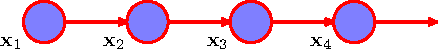
\includegraphics[]{figures/math/markov_chain}
  \caption{A graph model that represents the Markov chain.}
  \label{fig:mchain}
\end{figure}

\begin{figure}[p]
  \centering 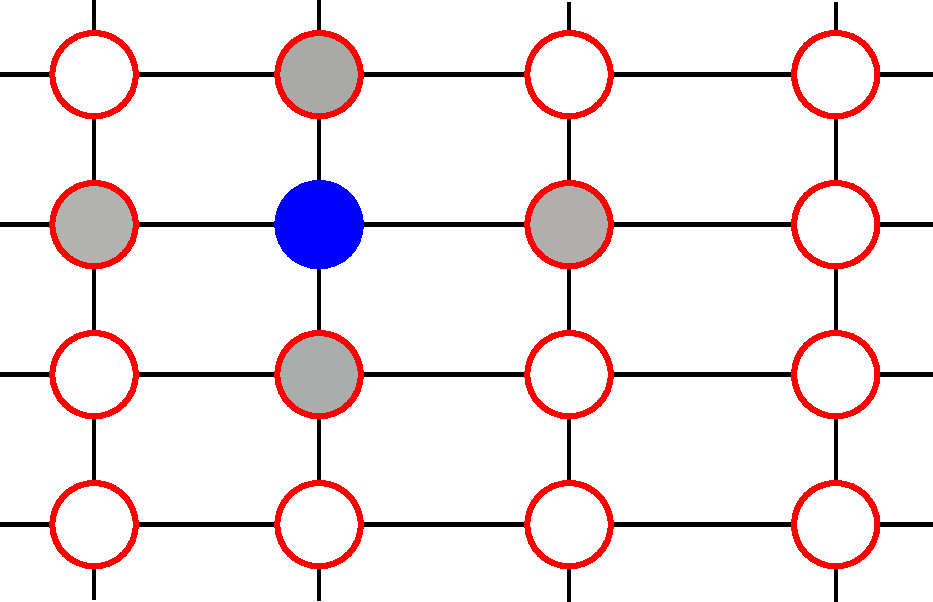
\includegraphics[width = 0.4\textwidth]{figures/math/mrf}
  \hspace{5pt} \includegraphics[width =
    0.4\textwidth]{figures/math/general_graph}
    \caption{Two graphical models represented by graphs. A graphical model
      representing a MRF can be either a regular grid or an general graph. For
      the regular grid, The node in blue color is conditional independent of
      the white node given it's adjacent neighbors, colored gray. For the
      general graph example, the two nodes in blue color are conditional
      independent given the remaining nodes. }
  \label{fig:mrf}
\end{figure}

\begin{figure}[p]
  \centering \includegraphics[width=0.5\textwidth]{figures/math/imagechain}
  \caption{A simulation of MRF. When a new candidate $w$ is accepted to replace
    current $x_s$, we get a new set of variables $X^{m+1}$ that differs from the
    current variable $X$ at only $s$. The set of variable $X^m$ and $W^{m+1}$
    is a sample of a Markov chain, since $X^{m+1}$ depends only on the previous
    $X^m$. Upon convergence, $X$ will be a sample from the target distribution
    $P(X)$. }
  \label{fig:imagechain}
\end{figure}

\begin{figure}[p]
  \centering
  \begin{subfigure}[b]{0.3\textwidth}
    \centering
    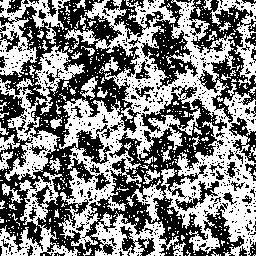
\includegraphics[width=\textwidth]{figures/math/ising_sim/b08_1000}
    \caption{$\beta = 0.8$}
    \label{fig:beta0.8}
    \end{subfigure}
~
  \begin{subfigure}[b]{0.3\textwidth}
    \centering
    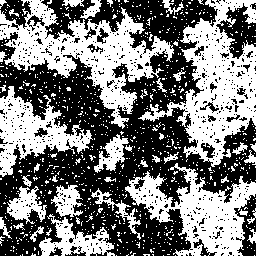
\includegraphics[width=\textwidth]{figures/math/ising_sim/b088_500}
    \caption{$\beta = 0.88$}
    \label{fig:beta0.88}
    \end{subfigure}
~
  \begin{subfigure}[b]{0.3\textwidth}
    \centering
    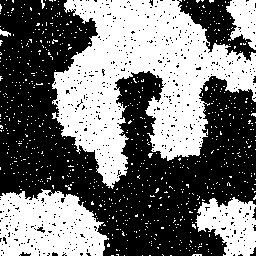
\includegraphics[width=\textwidth]{figures/math/ising_sim/b10_1000}
    \caption{$\beta = 1.0$}
    \label{fig:beta1.0}
    \end{subfigure}

  \begin{subfigure}[b]{0.3\textwidth}
    \centering
    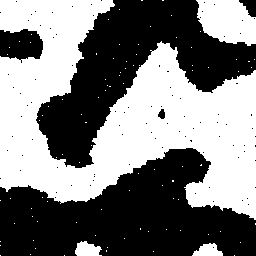
\includegraphics[width=\textwidth]{figures/math/ising_sim/b15_800}
    \caption{$\beta = 1.5$}
    \label{fig:beta1.5}
    \end{subfigure}
~
  \begin{subfigure}[b]{0.3\textwidth}
    \centering
    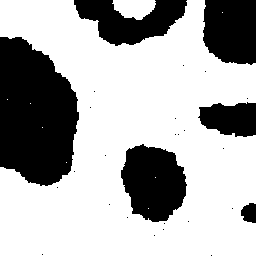
\includegraphics[width=\textwidth]{figures/math/ising_sim/b20_1000}
    \caption{$\beta = 2.0$}
    \label{fig:beta2.0}
    \end{subfigure}
~
  \begin{subfigure}[b]{0.3\textwidth}
    \centering
    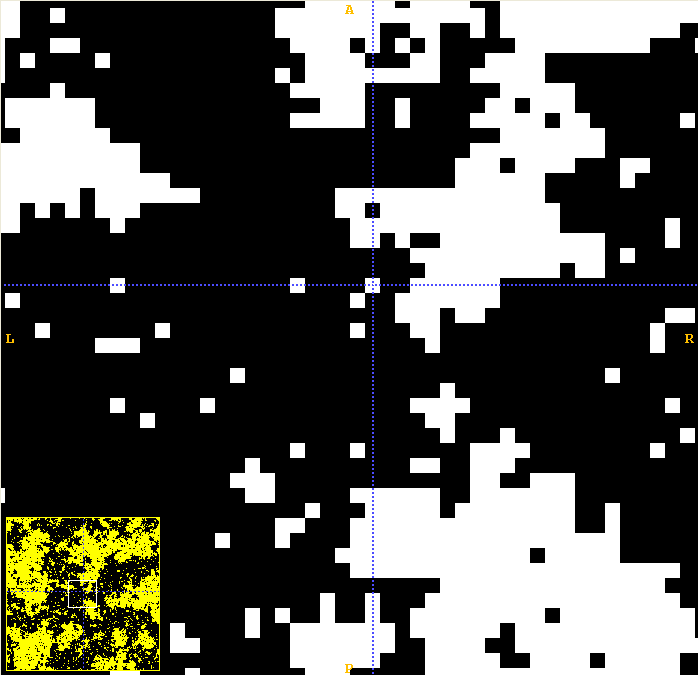
\includegraphics[width=\textwidth]{figures/math/ising_sim/b088_details}
    \caption{$\beta = 0.88$ zoomed in}
    \label{fig:beta0.88details}
    \end{subfigure}
  \caption{Simulating Ising model with various values of $\beta$. For each
    simulation, the image is initialized with random states, and then scanned
    1000 times. Notice when $\beta$ is small, the image is less spatially
    coherent. When $\beta$ is large, the image has more spatial coherent
    regions. }
  \label{fig:isingsim}
\end{figure}

\begin{figure}[p]
  \centering
  \begin{subfigure}[b]{0.3\textwidth}
    \centering 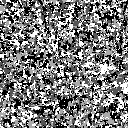
\includegraphics[width=\textwidth]{figures/math/potts_sim/b088}
    \caption{$\beta = 0.88$}
    \end{subfigure}
~
  \begin{subfigure}[b]{0.3\textwidth}
    \centering 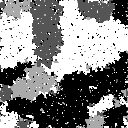
\includegraphics[width=\textwidth]{figures/math/potts_sim/b12}
    \caption{$\beta = 1.2$}
    \end{subfigure}
~
  \begin{subfigure}[b]{0.3\textwidth}
    \centering 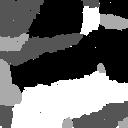
\includegraphics[width=\textwidth]{figures/math/potts_sim/b20}
    \caption{$\beta = 2.0$}
    \end{subfigure}
  \caption{Simulating Potts model of four states with various values of
    $\beta$. For all simulations, the image was initialized with random states,
    and then was scanned 1000 times. }
  \label{fig:pottssim}
\end{figure}

\begin{figure}[p]
  \centering 
  \begin{subfigure}[b]{\textwidth}
    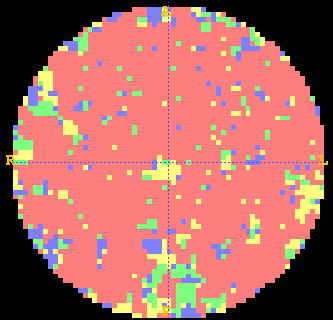
\includegraphics[width=0.3\textwidth]{figures/math/sw/gibbs1}
    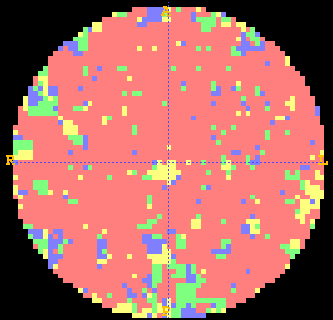
\includegraphics[width=0.3\textwidth]{figures/math/sw/gibbs2}
    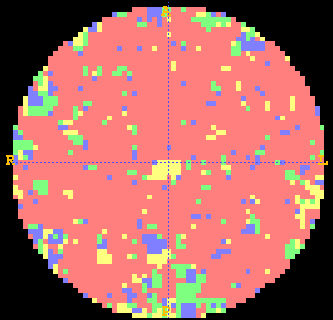
\includegraphics[width=0.3\textwidth]{figures/math/sw/gibbs3}
    \caption{Gibbs samples}
  \end{subfigure}
  ~
  \begin{subfigure}[b]{\textwidth}
    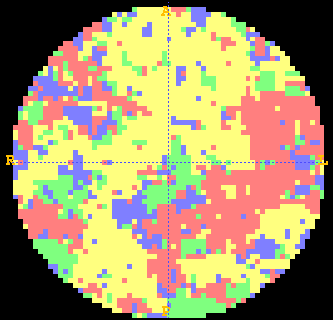
\includegraphics[width=0.3\textwidth]{figures/math/sw/sw1}
    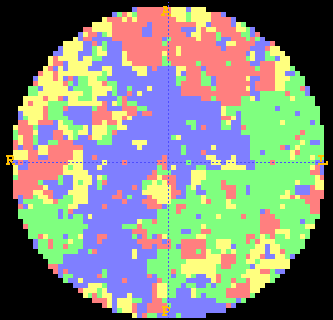
\includegraphics[width=0.3\textwidth]{figures/math/sw/sw2}
    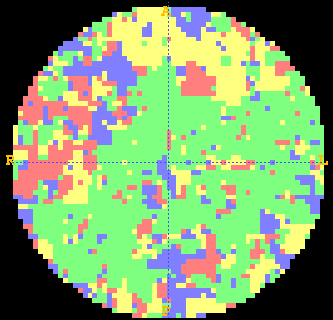
\includegraphics[width=0.3\textwidth]{figures/math/sw/sw3}
    \caption{SW samples}
    \end{subfigure}
    \caption{Consecutive samples of Potts model with $\beta = 1.1$ using SW
      and Gibbs sampling.  Both samplers initialize the sample image with
      all-zero values, have 100 burn-in sampling and then save three
      consecutive samples. Note for the SW samples, multiple voxel labels have
      been changed between the consecutive sample images. Such multiple
      updates speed up convergence. For Gibbs, the three sample images are
      similar due to the strong interactions (relatively large $\beta$)
      between the neighboring nodes. }
  \label{fig:mathsw}
\end{figure}

\begin{figure}[p]
  \centering \includegraphics[width = 0.5\textwidth]{figures/math/hmm}
  \caption{A graphical representation of the hidden Markov model(HMM). $X$ is
    defined on a regular lattice graph  and is given a MRF prior to represent
    our knowledge of the smoothness or piecewise constant. $Y$ is the observed
    data that is generated from the likelihood function given the hidden $X$.}
  \label{fig:hmm}
\end{figure}

\begin{figure}[p]
  \centering 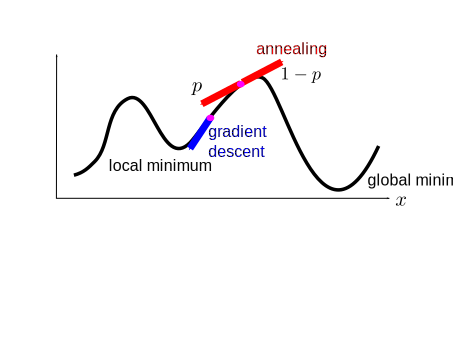
\includegraphics[width=0.6\textwidth]{figures/math/annealing}
  \caption{Simulated annealing samples one variable at a time. Unike
    coordinate descent that always moves in the gradient descent direction
    (blue color arrow), the SA algorithm updates the variable based on a certain
    probability, which depends on the difference of the function value of two
    configurations (red arrow).}
  \label{fig:annealing}
\end{figure}

\begin{figure}[p]
  \centering 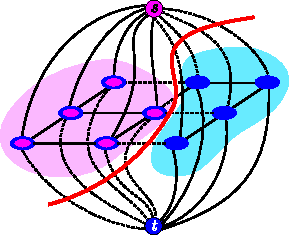
\includegraphics[width=0.5\textwidth]{figures/math/graphcuts}
  \caption{Graph cut segmentation. Each voxel is defined as a node on a
    graph. Neighboring voxels have edges between them with weights given by
    MRF. A source node $s$ and a sink node $t$ are added. All nodes have links to
    both sources and sink nodes with weights depend on the likelihood function
    (data term). Graph cut algorithms find a cut, i.e., a set of edges whose
    overall weights are minimized. In the figure, edges with solid lines are
    kept, and edges with dashed lines are removed after the cut. Red think links
    are the cut. Node is assigned to source or sink label if they are connected
    to either of them. }
  \label{fig:graphcuts}
\end{figure}

\begin{figure}[p]
  \centering 
  \begin{subfigure}[b]{0.3\textwidth}
  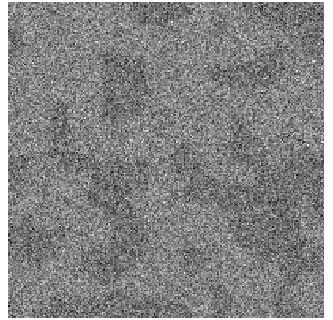
\includegraphics[width=1\textwidth]{figures/math/gc/obs}
  \caption{Observed noise image}
  \end{subfigure}
~
  \begin{subfigure}[b]{0.3\textwidth}
  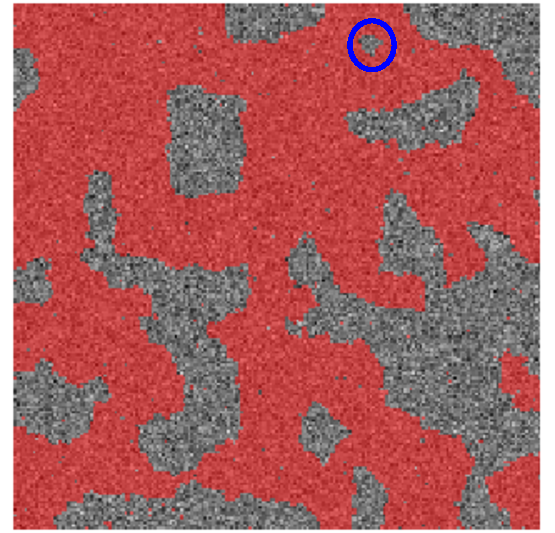
\includegraphics[width=1\textwidth]{figures/math/gc/truth_marked}
  \caption{Ground truth label map}
  \end{subfigure}
~
  \begin{subfigure}[b]{0.3\textwidth}
    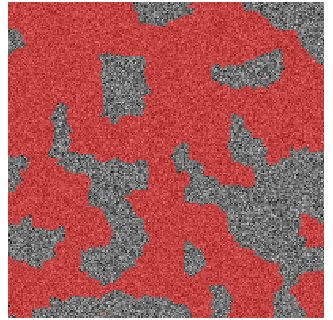
\includegraphics[width=1\textwidth]{figures/math/gc/rec}
    \caption{Recovered label map}
  \end{subfigure}


  \begin{subfigure}[b]{1\textwidth}
    \centering
    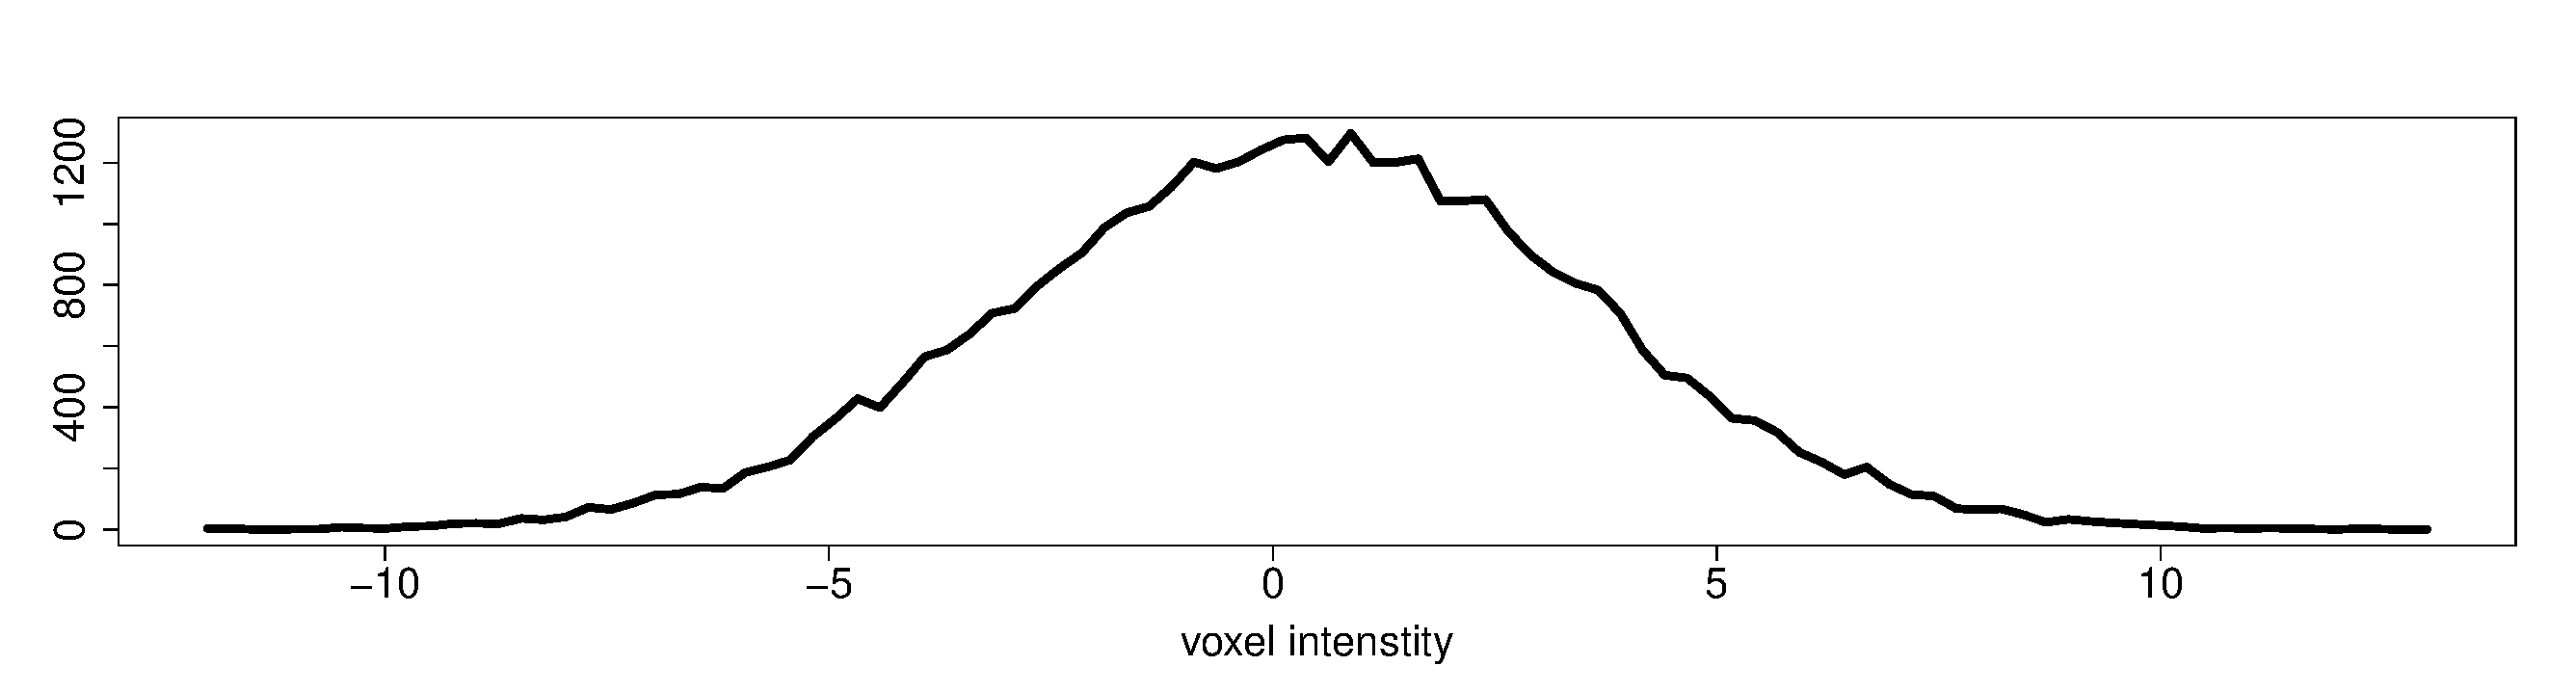
\includegraphics[width=0.8\textwidth]{figures/math/gc/hist}
    \caption{Histogram}
  \end{subfigure}

  \caption{Recovering noise image by graph cut. Top row from left to right:
    a) observed noised image, b) ground truth label map, c) recovered label
    map. Bottom d) histogram of the observed image intensity. Note the region in
    blue circle of the true map is misclassified. }
  \label{fig:gcexample}
\end{figure}

\begin{figure}[p]
  \centering 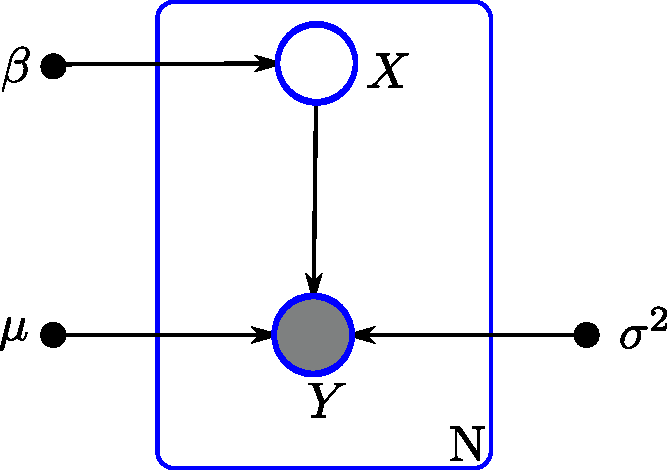
\includegraphics[width = 0.3\textwidth]{figures/math/paraest}
  \caption{A hidden Markov model with $X$ in MRF, and each $y_s$ is independent
    Gaussian given $x_s$. The parameters are black dots, the hidden variables
    are circles, and the observed data are grayed circles. The MRF structure on
    $X$ is not shown in this diagram. Instead a box is on $X$ and $Y$ to
    represent that there are $N$ such nodes. }
  \label{fig:paraest}
\end{figure}

\begin{figure}[p]
  \centering 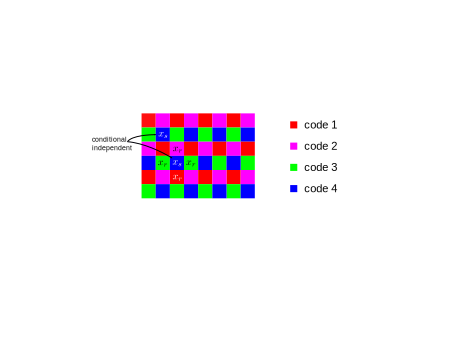
\includegraphics[width = 0.6\textwidth]{figures/math/coding}
  \caption{Coding scheme for parameter estimation. For four-neighbors system of two-dimensional
    image, the voxels are separated into four groups. The voxels in the same group
    are conditionally independent given other groups.}
  \label{fig:coding}
\end{figure}

\begin{figure}[p]
  \centering 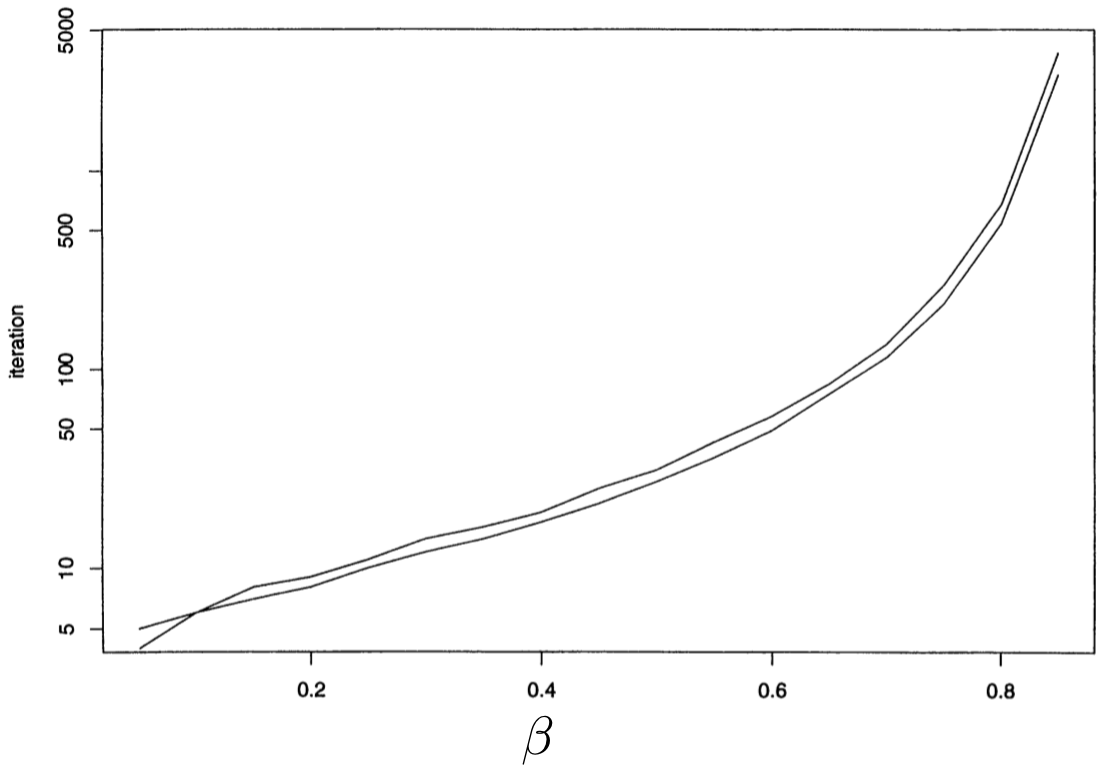
\includegraphics[width=0.7\textwidth]{figures/discussion/ising}
  \caption{Percentile of coupling iterations for Ising model of size $64\times
    64$. Top curve shows the 99\% and bottom shows the 95\% percentile from the
    distribution of the iterations needed for coupling, as a function of $\beta$
    parameter.  The percentiles are estimated using 1000 repetitions of Gibbs
    sampling initialized with all-white and all-black value. (adapted from
    Johnson~\cite{johnson1996studying}. }
\label{fig:ising}
\end{figure}

%%% Local Variables: 
%%% TeX-master: "MyThesis"
%%% End: 
